% Authors:
% M. Weyland (2020)
% A. Weyland (2020)
% H. Baur (2020)

\documentclass[twoside,a4paper,11pt,halfparskip,DIV=11,notitlepage]{scrartcl}
\usepackage{scrpage2}
\usepackage{amsmath}
\usepackage[pdfauthor={},pdftitle={},pdfstartview=FitH,pdfborder={0 0 0}]{hyperref}
\usepackage[ngerman]{babel}
\usepackage{babelbib}
\usepackage{float}
\usepackage{tikz}
\usetikzlibrary{positioning,arrows}
\usepackage[european]{circuitikz}
\usepackage{pgfplots}
\pgfplotsset{compat=1.16}
\usepgfplotslibrary{smithchart}

\usepackage{ccicons}
\usepackage{siunitx}
\usepackage{booktabs}
\usepackage{pifont}
\usepackage{xspace}
\DeclareUnicodeCharacter{2460}{\ding{172}\xspace}
\DeclareUnicodeCharacter{2461}{\ding{173}\xspace}
\renewcommand{\textdegree}{\si{\degree}\xspace}

\definecolor{HB9UFblue}{RGB}{0,61,165}
\definecolor{HB9UFred}{HTML}{ED135A}

\definecolor{marker}{HTML}{f9f871}
\definecolor{stimulus}{HTML}{ffc75f}
\definecolor{cal}{HTML}{ff9671}
\definecolor{recall}{HTML}{ff6f91}
\definecolor{config}{HTML}{d65db1}
% Spare color: #845ec2
\definecolor{trace0}{RGB}{255,200,0}
\definecolor{trace1}{RGB}{0,155,255}
\definecolor{trace2}{RGB}{0,220,0}
\definecolor{trace3}{RGB}{220,0,220}

\newcommand{\uline}[1]{%
    \tikz[baseline=(todotted.base)]{
        \node[inner sep=1pt,outer sep=0pt] (todotted) {#1};
        \draw[color=HB9UFblue,thick] (todotted.south west) -- (todotted.south east);
    }%
}%

\newcommand{\udash}[1]{%
    \tikz[baseline=(todotted.base)]{
        \node[inner sep=1pt,outer sep=0pt] (todotted) {#1};
        \draw[dashed,color=HB9UFred,thick] (todotted.south west) -- (todotted.south east);
    }%
}%

\newcommand{\Ohm}{$\Omega$\xspace}

\newcommand*\cleartoleftpage{%
  \clearpage
  \ifodd\value{page}\hbox{}\newpage\fi
}

\title{NanoVNA Primer}
\author{\sf UHF-Gruppe der USKA}
\date{\sf Version 0.3, CC BY-SA 4.0 \ccbysa}
\pagestyle{scrheadings}
%\setkomafont{pagehead}{\sf}

\usepackage{tikz}

%\setcounter{secnumdepth}{0} % sections are level 1

\sloppy

\begin{document}
\maketitle
\thispagestyle{empty}

\setcounter{tocdepth}{1}
\tableofcontents

%\vspace{2cm}

%\hfill
\includegraphics[width=2cm]{figures/hb9uf_logo.pdf}

\newpage

% FIXME: Einleitung

\section{Grundlagen}

\subsection{Ports, Reflexions- und Transmissionsmessung}\label{sec:ports}
Netzwerkanalysatoren sind Geräte, mit denen Transmissions- und
Reflexionseigenschaften von Hochfrequenznetzwerken frequenzabhängig ermittelt
werden können. Sie dienen dem Ausmessen von Antennen, Filtern, Transformatoren,
Baluns, Matching-Netzwerken, Splittern, Verstärkern, Stubs und vielem mehr. Ein
vollwertiger Netzwerkanalysator hat zwei Anschlüsse (sogenannte Ports), ① und ②.
Das Gerät kann sowohl an Port ① als auch an Port ② ein Prüfsignal (einen 
Stimulus) generieren. Bei aktiviertem Stimulus wird gemessen, wie viel des
Signals reflektiert wird (also in den aussendenden Port zurück gelangt), und
wie viel davon das zu testende Netzwerk durchwandert und zum jeweils anderen
Port gelangt (Transmission).

Viele Geräte -- darunter auch der NanoVNA -- implementieren vielfach nur einen Teil
dieser Messungen. Manchmal kommt der Stimulus nur aus einem der beiden Ports
und der Prüfling muss von Hand umgedreht werden; oder es sind nur
Reflexionsmessungen möglich, letzteres z.B. bei einem Antennen-Analyzer. So
oder so wird entweder nur die Amplitude (skalar) oder die Amplitude und Phase
(Vektor) gemessen (siehe Abschnitt \ref{sec:vectors}).

Die Reflexions- und die Transmissionsmessung sind in
Abbildung \ref{fig:testset} schematisch dargestellt: Ein aus Port ① ausgehender
Stimulus trifft auf einen Prüfling (ein Filter, eine Antenne etc.). Ein Teil
der eintreffenden Energie wird zurück zu Port ① reflektiert und dort gemessen
(Reflexionsmessung). Der Rest wird entweder vom Prüfling in Wärme umgewandelt,
als Radiowelle abgestrahlt oder gelangt (falls vorhanden) an den Ausgang des
Prüflings. Die Energie am Ausgang des Prüflings wird Port ② zugeführt
und dort gemessen (Transmissionsmessung).

\begin{figure}[H]
    \begin{center}
        \begin{tikzpicture}[text width=6em, text centered,, node distance=8em]
            \tikzstyle{box}=[draw,rounded corners=3pt,minimum height=3em]
            \node[box] (p1) {\sf\Large{Port ① \small{(CH0)}}};
            \node[box,right=of p1] (dut) {\sf\Large{DUT}};
            \node[box,right=of dut] (p2) {\sf\Large{Port ② \small{(CH1)}}};

            \draw[-stealth',thick,transform canvas={yshift=2mm}] (p1) -- node[above] {\sf Stimulus} (dut);
            \draw[-stealth',thick,transform canvas={yshift=-2mm}] (dut) -- node[below]{\sf Reflexion} (p1);
            \draw[-stealth',thick] (dut) -- node[above] {\sf Transmission} (p2);
        \end{tikzpicture}
    \end{center}
    \caption{Ein aus Port ① ausgehender Stimulus trifft auf einen Prüfling (device under test (DUT), z.B
        ein Filter, eine Antenne etc.). Ein Teil der eintreffenden Energie wird zurück zu Port ① reflektiert
        (Reflexionsmessung). Der Rest wird entweder vom Prüfling in Wärme umgewandelt, als Radiowelle
        abgestrahlt oder gelangt (falls vorhanden) an den Ausgang des Prüflings. Die Energie am Ausgang
        des Prüflings wird Port ② zugeführt und dort gemessen (Transmissionsmessung). Die Begriffe ``CH0''
        und ``CH1'' beziehen sich auf den NanoVNA und sind ansonsten unüblich.}
    \label{fig:testset}
\end{figure}

\subsection{Rückführungsdämpfung, Einfügedämpfung und Standing Wave Ratio}

Die durch Reflexion zurückgeführte Leistung wird mit der Leistung des Stimulus verglichen. Reflektiert
der Prüfling die gesamte Leistung, so erhält Port ① genausoviel Leistung zurück, wie er im Stimulus
ausgesandt hat (Kabeldämpfungen werden durch Kalibrierung korrigiert und sind deshalb hier vernachlässigt,
siehe Abschnitt \ref{sec:calibration}). Da die beiden Leistungen gleich gross sind, spricht man von
einer Rückführungsdämpfung von 0~dB. Reflektiert der Prüfling die halbe Leistung des Stimulus so spricht
man von einer Rückführungsdämpfung von 3~dB. Oft wird die Rückführungsdämpfung negativ angegeben, also
in diesem Fall -3~dB, was nicht ganz korrekt ist - es handelt sich ja schliesslich um eine Dämpfung 
und -3~dB Dämpfung wären +3~dB Verstärkung, was in dieser passiven Situation nicht eintreten kann.
Im Folgenden wird diese Konvention trotzdem verwendet, weil sie sich eingebürgert hat.

Das im Amateurfunk beliebte Stehwellenverhältnis (standing wave ratio, SWR) bezeichnet eigentlich
ein Amplitudenverhältnis von speziellen Stellen entlang einer Leitung (z.B. Koaxialkabel oder
Hühnerleiter). Bei der Bestimmung des SWR wird aber in den seltensten Fällen die Leitung an sich
untersucht. Oft ist die Leitung auch derart kurz, dass diese speziellen Stellen gar nicht auftreten.
Der Begriff ist deshalb leider etwas fehlgeleitet. Tatsächlich wird in aller Regel die Rückführungsdämpfung
gemessen und mit den entsprechenden Formeln in ein Stehwellenverhältnis umgesetzt. Tabelle \ref{tab:rlswr}
gibt den Zusammenhang zwischen Rückführungsdämpfung und SWR für ausgewählte Grössen an.

\begin{table}[H]
    \caption{Gegenübertellung von SWR, Rückführungsdämpfung und dem prozentualen Anteil reflektierter Leistung.}
    \label{tab:rlswr}
\begin{center}\begin{tabular}{SSS}\toprule
{\textbf{SWR}} & {\textbf{Rückführung}} & {\textbf{\% Reflkt.}}\\\midrule
1.0 & {-$\infty$} & 0.0\\
1.1 & -26.44 & 0.2\\
1.2 & -20.83 & 0.8\\
1.3 & -17.69 & 1.7\\
1.4 & -15.56 & 2.8\\
1.5 & -13.98 & 4.0\\
1.6 & -12.74 & 5.3\\
1.7 & -11.73 & 6.7\\
1.8 & -10.88 & 8.2\\
1.9 & -10.16 & 9.6\\
2.0 & -9.54 & 11.1\\
2.2 & -8.52 & 14.1\\
2.4 & -7.71 & 17.0\\
2.6 & -7.04 & 19.8\\
2.8 & -6.49 & 22.4\\\bottomrule
\end{tabular}
\hspace{1cm}
\begin{tabular}{SSS}\toprule
{\textbf{SWR}} & {\textbf{Rückführung}} & {\textbf{\% Reflkt.}}\\\midrule
3 & -6.02 & 25.0\\
4 & -4.44 & 36.0\\
5 & -3.52 & 44.4\\
6 & -2.92 & 51.0\\
7 & -2.5 & 56.3\\
8 & -2.18 & 60.5\\
9 & -1.94 & 64.0\\
10 & -1.74 & 66.9\\
20 & -0.87 & 81.9\\
30 & -0.58 & 87.5\\
40 & -0.43 & 90.6\\
50 & -0.35 & 92.3\\
60 & -0.29 & 93.5\\
80 & -0.22 & 95.1\\
100& -0.17 & 96.2\\\bottomrule
\end{tabular}\end{center}
\end{table}

Eine andere Darstellung des selben Zusammenhangs ist im Nomogramm in Abbildung
\ref{fig:rlnomogramm} zu sehen.

\begin{figure}[t]
    \begin{center}\begin{tikzpicture}[scale=1.25]
        % Return loss
        % [13, 10, 8.5, 7.5, 6.5, 5.5, 4.5, 3.5, 2.5, 1.5, 0.9, 0.7, 0.5, 0.3, 0.1]
        % [9, 8, 7, 6, 5, 4, 3, 2, 1, 0.8, 0.6, 0.4, 0.2, 0]
        % for i in y1: print("%.1f / %f, " % (i,  10**(-i/10)),)
        \foreach \rl/\x in {13 / 0.050119, 10 / 0.1, 8.5 / 0.141254, 7.5 / 0.177828, 6.5 / 0.223872, 5.5 / 0.281838, 4.5 / 0.354813, 3.5 / 0.446684, 2.5 / 0.562341, 1.5 / 0.707946, 0.9 / 0.812831, 0.7 / 0.851138, 0.5 / 0.891251, 0.3 / 0.933254, 0.1 / 0.97723}
        {
            \node[above] at ({\x*10},0.) {\sf\tiny{\rl}};
            \draw ({\x*10},0.05) -- ({\x*10},-0.05);
        }
        \foreach \rl/\x in { 9 / 0.125893, 8 / 0.158489, 7 / 0.199526, 6 / 0.251189, 5 / 0.316228, 4 / 0.398107, 3 / 0.501187, 2 / 0.630957, 1 / 0.794328, 0.8 / 0.831764, 0.6 / 0.870964, 0.4 / 0.912011, 0.2 / 0.954993, 0 / 1.000000}
        {
            \node[below] at ({\x*10},0.) {\sf\tiny{\rl}};
            \draw ({\x*10},0.05) -- ({\x*10},-0.05);
        }
        \node[above] at (0,0) {\sf\tiny{$\infty$}};
        \draw (0,0.05) -- (0,-0.05);
        \draw (0,0) -- (10,0);
        \node[right] at (10,0) {~\sf\scriptsize{RL (dB)}};

        % SWR
        % [1, 1.5, 1.9, 2.5, 3.5, 4.5, 5.5, 6.5, 7.5, 8.5, 9.5, 12, 16, 20, 40]
        % [1.3, 1.7, 2, 3, 4, 5, 6, 7, 8, 9, 10, 14, 18, 30, 50]
        %for i in x: print("%.1f / %f, " % (i,  ((i-1) / (i+1))**2 ))
        \begin{scope}[yshift=-20]
        \foreach \s/\x in {1.0 / 0.000000, 1.5 / 0.040000, 1.9 / 0.096314, 2.5 / 0.183673, 3.5 / 0.308642, 4.5 / 0.404959, 5.5 / 0.479290, 6.5 / 0.537778, 7.5 / 0.584775, 8.5 / 0.623269, 9.5 / 0.655329, 12 / 0.715976, 16 / 0.778547, 20 / 0.818594, 40 / 0.904819}
        {
            \node[above] at ({\x*10},0.) {\sf\tiny{\s}};
            \draw ({\x*10},0.05) -- ({\x*10},-0.05);
        }
        \foreach \s/\x in {1.3 / 0.017013, 1.7 / 0.067215, 2 / 0.111111, 3 / 0.250000, 4 / 0.360000, 5 / 0.444444, 6 / 0.510204, 7 / 0.562500, 8 / 0.604938, 9 / 0.640000, 10 / 0.669421, 14 / 0.751111, 18 / 0.800554, 30 / 0.875130, 50 / 0.923106 }
        {
            \node[below] at ({\x*10},0.) {\sf\tiny{\s}};
            \draw ({\x*10},0.05) -- ({\x*10},-0.05);
        }
        \node[above] at (10,0) {\sf\tiny{$\infty$}};
        \draw (10,0.05) -- (10,-0.05);
        \draw (0,0) -- (10,0);
        \node[right] at (10,0) {~\sf\scriptsize{SWR}};
        \end{scope}

        % Reflected power [%]
        \begin{scope}[yshift=-40]
         \foreach \x in {0,10,20,...,100}
         {
             \node[above] at ({\x/10},0.) {\sf\tiny{\x}};
             \draw (\x/10,0.05) -- (\x/10,-0.05);
         }
        \draw (0,0) -- (10,0);
        \node[right] at (10,0) {~\sf\scriptsize{\% Reflkt.}};
        \end{scope}
    \end{tikzpicture}\end{center}
    \caption{Nomogramm des Zusammenhangs zwischen Rückfürungsdämpfung (return loss, RL),
    Stehwellenverhältnis (standing wave ratio, SWR) und dem Anteil der reflektierten Leistung (\% Reflkt.).}
    \label{fig:rlnomogramm}
\end{figure}


Die Einfügedämpfung ist ebenfalls ein Leistungsverhältnis: Die Leistung, die
bei eingesetztem Prüfling zu Port ② gelangt wird verglichen mit der Leistung
in Port ②, wenn der Prüfling nicht eingesetzt ist. Dieser Sachverhalt ist in
Abbildung \ref{fig:insertionloss} dargestellt. Die Einfügedämpfung ist dabei
definiert als $d=P_b/P_a$ bzw $10\cdot\log{(d)}$ in Dezibel. Daraus wird erkennbar,
dass ein ``perfekt transparenter'' Prüfling eine Einfügedämpfung von 0~dB
hat. Sorgt ein Prüfling dafür, dass nur noch die halbe Leistung zu Port ②
gelangt, so hat er eine Einfügedämpfung von 3~dB usw. Auch hier wird manchmal
die Einfügedämpfung salopperweise negativ angegeben, was eigentlich falsch ist.

\begin{figure}[H]
    \begin{center}
        \begin{tikzpicture}[text width=5em,text centered,node distance=4em]
            \tikzstyle{box}=[draw,rounded corners=3pt,minimum height=2em]
            \node[box] (p1) {\sf{Port ①}};
            \node[box] (p2) at (10,0) {\sf{Port ②}, $P_a$};

            \draw[-stealth',thick] (p1) --  (p2);
        \end{tikzpicture}

        \vspace{5mm}

        \begin{tikzpicture}[text width=5em,text centered,node distance=4em]
            \tikzstyle{box}=[draw,rounded corners=3pt,minimum height=2em]
            \node[box] (p1) {\sf{Port ①}};
            \node[box] (dut) at (5,0) {\sf{DUT}};
            \node[box] (p2) at (10,0) {\sf{Port ②}, $P_b$};

            \draw[-stealth',thick] (p1) --  (dut);
            \draw[-stealth',thick] (dut) -- (p2);
        \end{tikzpicture}
    \end{center}
    \caption{Erklärung Einfügedämpfung: Die Leistung $P_a$ ohne Prüfling wird
    verglichen zur Leistung $P_b$ mit Prüfling (device under test, DUT).}
    \label{fig:insertionloss}
\end{figure}

\subsection{Reaktive Lasten}\label{sec:vectors}
Bis jetzt wurden sämtliche Überlegungen anhand von Verhältnissen zwischen
aus- und eingehenden Leistungen gemacht. Messungen dieser Grössen werden
skalare Messungen bezeichnet. Der NanoVNA bietet allerdings die Möglichkeit,
nicht nur skalar, sondern vektoriell zu arbeiten. Das bedeutet, dass er auch
Informationen über die Phase der ein- und ausgehenden Signale verarbeiten kann.

Dies ist im Zusammenhang mit reaktiven Elementen (Spule/Induktivität,
Kondensator/Kapazität, Antenne ausserhalb der Resonanz etc.) wichtig: Reaktive
Elemente haben einen Blindwiderstand, der in aller Regel frequenzabhängig ist.
Dies ist in Abbildung \ref{fig:XRLC} dargestellt: Der Blindwiderstand $X$ eines
Widerstandes $R$ ist $X_R=0~\Omega$ ungeachtet der Frequenz, der Blindwiderstand
einer (idealen) Induktivität $L$ nimmt mit der Frequenz $f$ zu ($X_L=2\pi f L$)
und der Blindwiderstand einer Kapazität $C$ nimmt mit zunehmender Frequenz $f$
ab ($X_C=(2\pi f C)^{-1}$).

Spulen und Kondensatoren sind in Bezug auf ihren Blindwiderstand duale Elemente:
Werden sie in Serie geschaltet, so wirken $X_L$ und $X_C$ entgegengesetzt, und
wenn beide gleich gross sind, dann heben sie sich genau auf. In einem
Schwingkreis oder einer Antenne ist dies genau bei Resonanz erfüllt (vgl. auch
Abbildung \ref{fig:resonanzplot} in Abschnitt \ref{sec:schwingkreis}). Weil
$X_L$ und $X_C$ entgegengesetzt wirken, wird der kapazitive Blindwiderstand
$X_C$ oft negativ angegeben. So wird erkennbar, ob der Blindwiderstand induktiv
oder kapazitiv ist. Auch über diese Konvention lässt sich debattieren.

\begin{figure}
    \begin{tikzpicture}
        \begin{axis}[
            title = {Widerstand},
            xmin=0, xmax=10,
            ymin=-100,ymax=500,
            grid=both,
            xlabel={Frequenz $f$/Hz},
            ylabel={\uline{Blindwiderstand $X/\Omega$}},
            xticklabels={},
            yticklabels={},
            ytick = {-400,-200,0,200,400},
            height=4cm,
            width=0.3\textwidth,
            major grid style={black!10}
        ]
        \addplot [mark=none,samples=100,domain=0:10,color=HB9UFblue,thick] {0};
        \end{axis}
        \begin{axis}[
            xmin=0, xmax=10,
            ymin=-100,ymax=500,
            grid=none,
            separate axis lines,
            ylabel style = {align=center},
            ticks=none,
            xmajorticks=true,
            xminorticks=false,
            ymajorticks=true,
            yminorticks=false,
            scaled ticks=false,
            xtick = {0},
            ytick = {0},
            axis y line*=right,
            height=4cm,
            width=0.3\textwidth,
            major grid style={black!10}
        ]
        \addplot [mark=none,samples=100,domain=0:10,color=HB9UFred,dashed,thick] {300};
        \end{axis}
    \end{tikzpicture}\hfill
    \begin{tikzpicture}
        \begin{axis}[
            title = {Induktivität},
            xmin=0, xmax=10,
            ymin=-100,ymax=500,
            grid=both,
            xlabel={Frequenz $f$/Hz},
            xticklabels={},
            yticklabels={},
            ytick = {-400,-200,0,200,400},
            height=4cm,
            width=0.3\textwidth,
            major grid style={black!10}
        ]
        \addplot [mark=none,samples=100,domain=0:10,color=HB9UFblue,thick] {40*x};
        \end{axis}
        \begin{axis}[
            xmin=0, xmax=10,
            ymin=-100,ymax=500,
            grid=none,
            separate axis lines,
            ylabel style = {align=center},
            ticks=none,
            xmajorticks=true,
            xminorticks=false,
            ymajorticks=true,
            yminorticks=false,
            scaled ticks=false,
            xtick = {0},
            ytick = {0},
            axis y line*=right,
            height=4cm,
            width=0.3\textwidth,
            major grid style={black!10}
        ]
        \addplot [mark=none,samples=100,domain=0:10,color=HB9UFred,dashed,thick] {0};
        \end{axis}
    \end{tikzpicture}\hfill
    \begin{tikzpicture}
        \begin{axis}[
            title = {Kapazität},
            xmin=0, xmax=10,
            ymin=-100,ymax=500,
            grid=both,
            xlabel={Frequenz $f$/Hz},
            xticklabels={},
            yticklabels={},
            ytick = {0,200,400},
            height=4cm,
            width=0.3\textwidth,
            major grid style={black!10}
        ]
        \addplot [mark=none,samples=100,domain=0.2:10,color=HB9UFblue,thick] {200/x};
        \end{axis}
        \begin{axis}[
            xmin=0, xmax=10,
            ymin=-100,ymax=500,
            grid=none,
            separate axis lines,
            ylabel style = {align=center},
            ylabel={\udash{Wirkwiderstand $R/\Omega$}},
            ticks=none,
            xmajorticks=true,
            xminorticks=false,
            ymajorticks=true,
            yminorticks=false,
            scaled ticks=false,
            xtick = {0},
            ytick = {0},
            axis y line*=right,
            height=4cm,
            width=0.3\textwidth,
            major grid style={black!10}
        ]
        \addplot [mark=none,samples=100,domain=0:10,color=HB9UFred,dashed,thick] {0};
        \end{axis}
    \end{tikzpicture}
    \caption{Blindwiderstand eines Widerstandes (Bauteil), einer Induktivität ($X_L$) und einer
    Kapazität ($X_C$) von links nach rechts. Der Wirkwiderstand ist jeweils gestrichelt gezeichnet.}
    \label{fig:XRLC}
\end{figure}

\subsection{Phasenverschiebung mit reaktiven Lasten}
Ein Spannungsteiler bestehend aus zwei 100~$\Omega$ (Wirk-)Widerständen
halbiert die Eingangspannung, bei Gleichspannung wie auch bei Wechselspannung.
Dieser Sachverhalt ist im oberen Teil von Abbildung \ref{fig:phasenverschiebung} festgehalten.
Es wäre nun naheliegend anzunehmen, dass man einen dieser beiden Widerstände
durch eine Induktivität oder Kapazität mit einem Blindwiderstand von 100~$\Omega$
ersetzen könnte und nach wie vor über einen Spannungsteiler verfügt, welcher
die Eingangsspannung halbiert, das ist allerdings nicht der Fall, wie Abbildung
\ref{fig:phasenverschiebung} aufzeigt: Oben erfolgt die Halbierung der Spannung
wie beschrieben. In der unteren Hälfte der Abbildung ist der 100~$\Omega$
Widerstand durch eine Spule ersetzt, welche bei der Testfrequenz von $f=$100~MHz
$X_L=100$~$\Omega$ aufweist. Dennoch weist $U_L$ mehr als die halbe Amplitude von
$U_Q$ auf; ausserdem wird die Phasenverschiebung sichtbar. Diese Beobachtungen
lassen eine Reihe von Schlussfolgerungen zu, die im Weiteren wichtig sein werden:

\begin{itemize}
    \item Die Blindwiderstände der betrachteten Komponenten sind frequenzabhängig,
        Wirkwiderstände sind es nicht.
    \item Blindwiderstände führen zu Phasenverschiebungen, Wirkwiderstände nicht.
    \item Wirk- und Blindwiderstände dürfen nicht ``einfach so'' miteinander
        verrechnet werden, denn das so gefundene Resultat mit dem Spannungsteiler 
        stimmt nicht mit dem Experiment überein. Wenn, dann gibt es strikte und
        offenbar nicht-triviale Regeln, wie gerechnet werden muss.
\end{itemize}

Übrigens hat eine Spule in der Praxis zusätzlich zu Blindwiderstand auch immer
selbst einen Wirkwiderstand, weil der Draht, aus dem sie gewickelt ist,
verlustbehaftet ist. 


\begin{figure}
    \scalebox{0.8}{\begin{circuitikz}
        \draw (0,0) to[sinusoidal voltage source=$U_Q$] (0,-4)
              (0,0) to[short] (3,0) to[R,a=100~$\Omega$] (3,-2) to[short,-o] (5,-2)
              (3,-2) to[R,a=100~$\Omega$,*-*] (3,-4) to[short,-o] (5,-4)
              (3,-4) to[short,-*] (0,-4) node[ground] {};
        \draw[-stealth',shorten >=3mm,shorten <=3mm] (5,-2) -- node[right]{$U_L$} (5,-4);
     \end{circuitikz}}
    \hfill
    \begin{tikzpicture}
        \begin{axis}[
            xmin=0, xmax=10,
            ymin=-1.25,ymax=1.25,
            ylabel={Spannung / V},
            grid=both,
            xlabel={Zeit / ns},
            yticklabels={},
            xtick = {0,2.5,5,7.5,10},
            ytick = {-1,-0.5,0,0.5,1},
            height=4cm,
            width=0.6\textwidth,
            major grid style={black!10}
        ]
        \addplot [mark=none,samples=100,domain=0:10,color=HB9UFblue,thick] {0.5*sin(3600*x)} node[below,pos=0.45] {$U_L$};
        \addplot [mark=none,samples=100,domain=0:10,color=HB9UFred,dashed,thick] {sin(3600*x)} node[above,pos=0.45] {$U_Q$};;
        \end{axis}
    \end{tikzpicture}

    \vspace{5mm}

    \scalebox{0.8}{\begin{circuitikz}
        \draw (0,0) to[sinusoidal voltage source=$U_Q$] (0,-4)
              (0,0) to[short] (3,0) to[R,a=100~$\Omega$] (3,-2) to[short,-o] (5,-2)
              (3,-2) to[L,a=160~nH,*-*] (3,-4) to[short,-o] (5,-4)
              (3,-4) to[short,-*] (0,-4) node[ground] {};
        \draw[-stealth',shorten >=3mm,shorten <=3mm] (5,-2) -- node[right]{$U_L$} (5,-4);
     \end{circuitikz}}
    \hfill
    \begin{tikzpicture}
        \begin{axis}[
            xmin=0, xmax=10,
            ymin=-1.25,ymax=1.25,
            ylabel={Spannung / V},
            grid=both,
            xlabel={Zeit / ns},
            yticklabels={},
            xtick = {0,2.5,5,7.5,10},
            ytick = {-1,-0.5,0,0.5,1},
            height=4cm,
            width=0.6\textwidth,
            major grid style={black!10}
        ]
        \addplot [mark=none,samples=100,domain=0:10,color=HB9UFblue,thick] {0.7*sin(3600*x+45)} node[below,pos=0.45] {$U_L$};
        \addplot [mark=none,samples=100,domain=0:10,color=HB9UFred,dashed,thick] {sin(3600*x)} node[above,pos=0.45] {$U_Q$};;
        \end{axis}
    \end{tikzpicture}
    \caption{Oben: Ein Spannungsteiler halbiert die Spannung: $U_L$ hat die
    halbe Amplitude von $U_Q$. Unten: Phasenverschiebung durch reaktives Element. Bei
einer Frequenz von $f=100$~MHz hat eine Induktivität von 160~nH genau
$X_L=100$~$\Omega$. Dennoch wird die Spannung nicht halbiert, stattdessen wird eine Phasenverschiebung sichtbar.}
    \label{fig:phasenverschiebung}
\end{figure}

\subsection{Das Smith-Diagramm}
Aus dem letzten Abschnitt wird klar: Die betrachteten Bauteile Widerstand, Kondensator und Spule haben Wirk- und
Blindwiderstände, und eine Serienschaltung aus einem Widerstand von
$R=100$~$\Omega$ und einer Spule mit einem Blindwiderstand von $X_L=100$~$\Omega$ hat nicht einen Ersatzwiderstand
von 100~$\Omega$. Bis auf weiteres werden Wirk- und Blindwiderstand als separate Grössen geführt. Ein Bauteil,
oder eine Kombination von Bauteilen, kann auf diese Art einen Wirkwiderstand
$R\ge0$, wie auch einen Blindwiderstand $X$ haben. Ist der Blindwiderstand positiv, so handelt es sich um ein
Induktivität; ein negativer Blindwiderstand beschreibt eine Kapazität. Für ein Bauteil oder eine Schaltung
aus Bauteilen kann also z.B. gelten: $R=200$~$\Omega$, $X=100$~$\Omega$. Diese Grösse wird Impedanz $Z$ genannt
und lässt sich in einem Koordinatensystem als Punkt darstellen, wenn $R$ auf
der horizontalen und $X$ auf der vertikalen Achse abgetragen wird. Das Beispiel
ist in Abbildung \ref{fig:euler} in  blau gezeichnet. 

Auch im Smith-Diagramm wird genau diese Information (also eine Impedanz bestehend aus Wirk- und Blindwiderstand)
ebenfalls als Punkt dargestellt. Ein Punkt im Smith-Diagramm unterscheidet sich in dieser Hinsicht also nicht
von einem Punkt im eingangs besprochenen Koordinaten-System. Der Unterschied ist lediglich, dass im Smith-Diagramm
die ``Achsen'' eine andere Form, welche auf den ersten Blick sehr sonderbar erscheinen mag. Punkt (und damit Impedanzen)
im Smith-Diagramm folgen diesen Regeln:


\begin{enumerate}
\item Üblicherweise wird das Smith-Diagramm auf 50~$\Omega$ normalisiert, so dass
    der Punkt genau in der Mitte $R=50$~\Ohm und $X=0$~\Ohm aufweist.
\item Auf der Horizontalen in der Mitte des Diagrammes sind alle Impedanzen mit $X=0$~\Ohm, also alle Impedanzen
    ohne Blindanteil.
\item Der Punkt ganz links auf dieser Horizontalen ist $R=0$~\Ohm, also eine Impedanz ohne Wirk- und Blindwiderstand
    bzw. ein Kurzschluss.
\item Der Punkt ganz rechts auf der selben Horizontalen ist $R=\infty$~\Ohm, also eine offene Verbindung.
\item Punkte oberhalb der Horizontalen sind induktive Impedanzen ($X>0$~\Ohm).
\item Punkte unterhalb der Horizontalen sind kapazitive Impedanzen ($X<0$~\Ohm).
\item Punkte auf der umgebenden Kreislinie haben keinen Wirkwiderstand, sie sind also rein induktiv bzw. kapazitiv.
\end{enumerate}

\begin{figure}[t]
    \begin{center}
        \begin{tikzpicture}
            \begin{axis}[
                xmin=-5, xmax=355,
                ymin=-155,ymax=155,
                xlabel={$R/\Omega$},
                ylabel={$X/\Omega$},
                grid=both,
                height=7cm,
                axis x line=center,
                axis y line=center,
                width=0.9\textwidth,
                major grid style={black!10}
            ]
            \fill [fill=HB9UFblue] (axis cs:200,100) circle [radius=3pt] node[right] {$R=200$~\Ohm, $X=100$\Ohm};
            \fill [fill=black] (axis cs:50,0) circle [radius=2pt] node[above right] {$R=50$~\Ohm, $X=0$~\Ohm};
            \fill [fill=black] (axis cs:0,100) circle [radius=2pt] node[right] {$R=0$~\Ohm, $X=100$~\Ohm (Spule)};
            \fill [fill=black] (axis cs:0,-100) circle [radius=2pt] node[right] {$R=0$~\Ohm, $X=-100$~\Ohm (Kondensator)};
            \fill [fill=black] (axis cs:0,0) circle [radius=2pt];
            \draw[stealth'-] (axis cs:5,5) -- (axis cs:40,40) node[above right] {$R=0$~\Ohm, $X=0$~\Ohm (Kurzschluss)};
        \end{axis}
        \end{tikzpicture}
    \end{center}
    \caption{Darstellung einer Impedanz mit $R=200$~$\Omega$ auf der horizontalen Achse und $X=100$~$\Omega$
    auf der vertikalen Achse (blau), sowie einer Reihe anderer Impedanzen (schwarz).}
    \label{fig:euler}
\end{figure}

In Abbildung \ref{fig:smithimpedance} sind die selben Impedanzen zu sehen wir in Abbildung \ref{fig:euler}, nur
sind sie nun in einem Smith-Diagramm dargestellt. Berechtigterweise stellt sich die Frage, wozu denn das Ganze
gut sein soll.

\begin{itemize}
    \item Richtung der Impedanzen, Matching
    \item Leitungstheoretische Aspekte
\end{itemize}

\begin{figure}
    \begin{tikzpicture}
        \begin{smithchart}[width=\textwidth,show origin code/.code={},clip=false,xticklabel style={font=\small},yticklabel style={font=\small}]
            \tikzstyle{note}=[align=center,fill=black]
            \fill [note,fill=HB9UFblue] (axis cs:4,2) circle [radius=4pt] node[above] {$R=200$~\Ohm, $X=100$\Ohm};
            \fill[note] (axis cs:1,0) circle [radius=3pt] node[below] {$R=50$~\Ohm, $X=0$~\Ohm};
            \fill[note] (axis cs:0,2) circle [radius=3pt] node[below left] {$R=0$~\Ohm, $X=100$~\Ohm\\ (Spule)};
            \fill[note] (axis cs:0,-2) circle [radius=3pt] node[above left] {$R=0$~\Ohm, $X=-100$~\Ohm\\ (Kondensator)};
            \fill[note] (axis cs:0,0) circle [radius=3pt] node[below right] {$R=0$~\Ohm, $X=0$~\Ohm\\ (Kurzschluss)};
            \fill[note] (axis cs:1000,1000) circle [radius=3pt] node[below left] {Offen};
        \end{smithchart}
    \end{tikzpicture}
    \caption{Smith-Diagramm der Impedanzen aus Abbildung \ref{fig:euler}.}
    \label{fig:smithimpedance}
\end{figure}

\subsection{Kalibrierung}\label{sec:calibration}

Zur Korrektur von Messabweichungen in Testkabeln und dem Gerät
(Frequenzabhängkeit von Stimulus und Detektor) muss vor jeder Messung eine
Kalibrierung durchgeführt werden. Wie in Abschnitt \ref{sec:tl} erläutert,
werden Impedanzen durch Leitungen transformiert. Eine Kalibrierung macht
auch diesen Effekt rückgängig. Dafür wird ein Kalibrierungs-Standard
(auch Kalibrierungskit genannt) benötigt; in Abbildung \ref{fig:calkit} ist
das Kalibrierungskit abgebildet, das mit dem NanoVNA geliefert wird. Es
besteht aus einer offenen Verbindung (``open''), einem Kurzschluss (``short''),
einem 50~\Ohm Abschluss (``load'') und einem Verbundungsstück (``thru'').
Es gibt eine ganze Reihe von Kalibrierungstechniken, welche z.B. in
\cite{hiebel2007fundamentals}  und \cite{hiebel2008vector} erklärt sind. In
den folgenden zwei Abschnitten werden für Reflexions- und Transmissionsmessung
je eine einfache Kalibrierung vorgestellt.

\begin{figure}[t]
    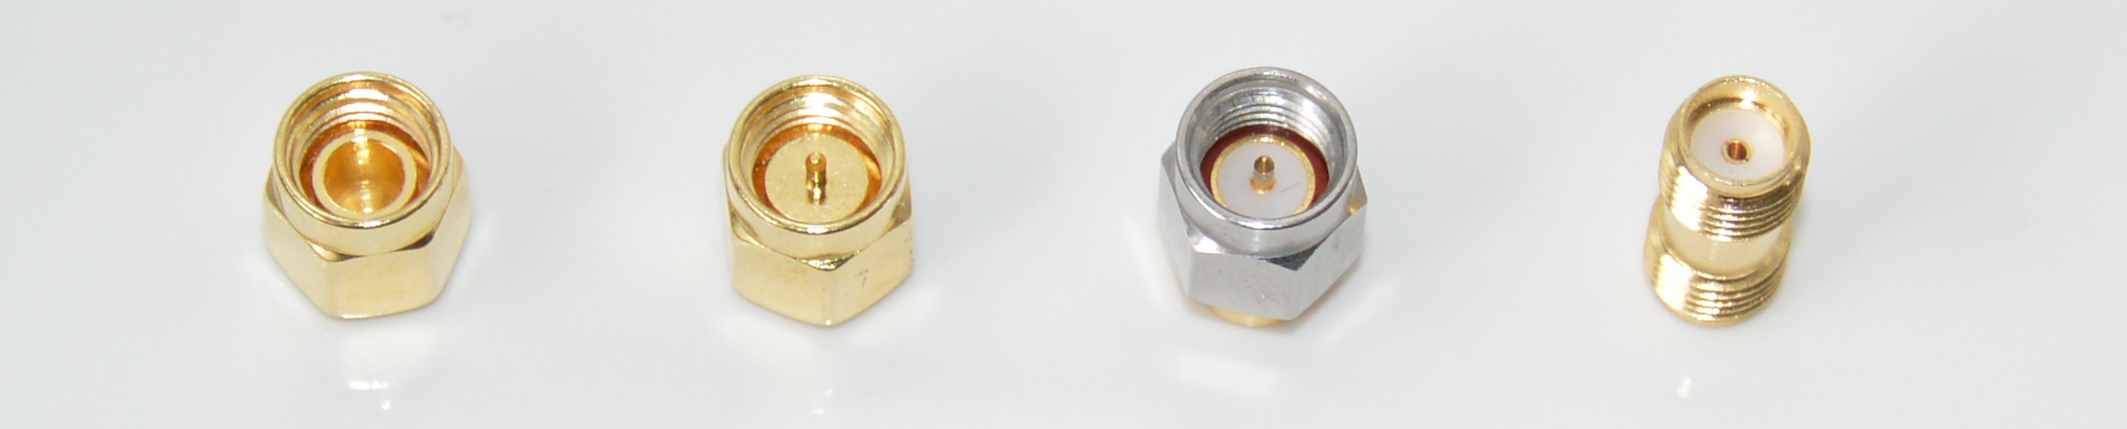
\includegraphics[width=\textwidth]{figures/calkit.jpg}
    \caption{NanoVNA Kalibrierungs-Standard. Von links nach rechts:
        Offenen Verbindung (``open''), Kurzschluss (``short''),
    50~\Ohm Abschluss (``load''), Verbundungsstück (``thru'').}
    \label{fig:calkit}
\end{figure}

\subsubsection{Reflexionsmessung}
Diese Messung wir mit einer offenen Verbindung (open, O), einem Kurzschluss
(short, S) und einer 50~\Ohm Last (load bzw. match, L/M) durchgeführt. Diese Art von
Kalibrierung wird deshalb auch OSL- bzw. OSM-Kalibrierung genannt. Diese
werden der Reihe nach angeschlossen und das Messgerät über den aktuell angeschlossenen
Abschluss orientiert. Dabei ist es wichtig, dass der Standard dort angeschlossen
wird, wo auch die Messung erfolgen soll. Das Gerät kann so die Transformation
der Messleitung sowie weitere Fehler rückgängig machen.

\subsubsection{Transmissionsmessung}
Bei der Transmissionsmessung wird das Gerät mit einem Verbindungsstück (thru, T) kalibriert,
welcher dann entfernt bzw. durch den Prüfling ersetzt wird. So weiss das  Gerät,
wieviel Energie in welcher Phase vom einen in den anderen Port gelangt, wenn der
Prüfling nicht eingeschleift wird. Diese Messung wird dann als 0~dB bzw. 0° Referenz
genutzt. Jeder Fehler im Verbindungsstück (Dämpfung $>$ 0~dB, Phasengang $\ne$~0°)
wirkt sich direkt auf die Messung aus.


\newpage % FIXME
\section{Bedienung NanoVNA}
Der NanoVNA wird mit einem Schiebe-Schalter ein- und ausgeschalten. Beim Einschalten
leuchtet eine blaue LED auf, welche nach dem Ausschalten noch bis zu einer Minute
nachleuchtet. Das Gerät wird über das mitgelieferte USB-C Kabel geladen. Die blaue
LED blinkt, bis der Akku voll ist, anschliessend hört sie auf zu blinken.
% FIXME: Leuchtet konstant oder ist erloschen?

Der grundsätzliche Messablauf ist immer gleich:

\begin{enumerate}
    \item Einstellung der Frequenz (Abschnitt \ref{sec:nanovnafreq})
    \item Kalibrierung (Abschnitt \ref{sec:nanovnacal})
    \item Anzeige von Spuren ein- und ausschalten (Abschnitt \ref{sec:nanovnatraces})
    \item Kanalwahl (Abschnitt \ref{sec:nanovnachannel} und Einstellung des Anzeigeformates
        (Abschnitt \ref{sec:nanovnaformat})
\end{enumerate}

Bei einer Änderung des Frequenzbereiches muss das Gerät für die bestmögliche Messung
rekalibriert werden.

Weil der Bildschirm etwas klein ist, lohnt sich die Bedienung mit Hilfe eines
Plastik-Stiftes. Der NanoVNA hat ein relativ umfangreiches Menü, welches in
Abschnitt \ref{sec:menu} als Referenz abgedruckt ist. Bei der üblichen Bedienung
finden aber immer wieder die selben Menüpunkte Anwendung.  Diese sind im
Folgenden erläutert.

\subsection{Einstellen des Frequenzbereiches}\label{sec:nanovnafreq}

\begin{center}\begin{tikzpicture}[font=\sffamily]
    \tikzstyle{menu}=[draw, text width=5em, text centered, minimum height=2em, node distance=2em,on grid]
    \tikzstyle{stimulus}=[fill=stimulus]
    \node[menu,stimulus] (stimulus) {Stimulus};
    \node[menu,stimulus,right=10em of stimulus] (start) {Start};
    \node[menu,stimulus,below of=start] (stop) {Stop};
    \node[menu,stimulus,below of=stop] (center) {Center};
    \node[menu,stimulus,below of=center] (span) {Span};
    \node[menu,stimulus,below of=span] (cwfreq) {CW Freq};
    \node[menu,stimulus,below of=cwfreq] (pausesweep) {Pause Swp.};
    \draw[thick,-stealth'] (stimulus) -- (start);
\end{tikzpicture}\end{center}


Der Frequenzbereich wird im Menü ``Stimulus'' eingestellt. Die kann auf zwei
Arten erfolgen:

\begin{itemize}
    \item Mit ``Start'' und ``Stop'' werden Anfangs- und Endfrequenz eingegeben. Eine Anfangsfrequenz von
        430~MHz und eine Endfrequenz von 440~MHz führen dazu, dass das  Gerät im Frequenzbereich von 430~MHz bis 440~MHz misst.
    \item Mit ``Center'' und ``Span'' wird die Mittefrequenz und Bandbreite eingegeben. Eine Mittefrequenz von 435~MHz
        und eine Bandbreite von 10~MHz führen also zur selben Messung wie oben.
\end{itemize}

Mit der Einstellung ``CW Freq'' wird das Gerät auf eine einzige Frequenz fixiert.
Der aktuelle Frequenzbereich wird im Display unten in der linken (Start) bzw.
rechten (Stop) Ecke angezeigt.
Für eine gute Messung muss nach einer Änderung des Frequenzbereiches unbedingt
rekalibriert werden (siehe Abschnitt \ref{sec:nanovnacal}). Eine erneute Kalibrierung
ist nach einer Änderung des Kanales (Abschnitt \ref{sec:nanovnachannel}) oder
des Anzeigeformates (Abschnitt \ref{sec:nanovnaformat}) nicht notwendig.

\subsection{Kalibrierung}\label{sec:nanovnacal}
\begin{center}\begin{tikzpicture}[font=\sffamily]
    \tikzstyle{menu}=[draw, text width=5em, text centered, minimum height=2em, node distance=2em,on grid]
    \tikzstyle{cal}=[fill=cal]
    \node[menu,cal,below of=stimulus] (cal) {Cal};
    \node[menu,cal,right=10em of cal] (calibrate) {Calibrate};
    \node[menu,cal,below of=calibrate] (calsave) {Save};
    \node[menu,cal,below of=calsave] (reset) {Reset};
    \node[menu,cal,below of=reset] (correction) {Correction};

    \node[menu,cal,right=20em of calibrate] (open) {Open};
    \node[menu,cal,below of=open] (short) {Short};
    \node[menu,cal,below of=short] (load) {Load};
    \node[menu,cal,below of=load] (isoln) {Isoln};
    \node[menu,cal,below of=isoln] (thru) {Thru};
    \node[menu,cal,below of=thru] (done) {Done};

    \node[menu,cal,right=10em of calsave] (save0) {Save 0};
    \node[menu,cal,below of=save0] (savei) {...};
    \node[menu,cal,below of=savei] (save4) {Save 4};

    \draw[thick,-stealth'] (cal) -- (calibrate);
    \draw[thick,-stealth'] (calibrate) -- (open);
    \draw[thick,-stealth'] (calsave) -- (save0);
\end{tikzpicture}\end{center}

Nach jeder Änderung des Frequenzbereiches oder des Messaufbaus sollte der
NanoVNA rekalibriert werden. Dafür ist das Menü ``Cal'' vorgesehen. Für die
Kalibrierung wird ein Kalibrierungskit (siehe Abschnitt \ref{sec:calibration}
und Abbildung \ref{fig:calkit}) benötigt. Eine Kalibrierung für die
Reflexionsmessung beinhaltet folgende Schritte:

\begin{enumerate}
    \item Im Menü ``Cal'' das Feld ``Reset'' wählen.
    \item Das Untermenü ``Calibrate'' wählen.
    \item Den offenen Abschluss befestigen und ``Open'' wählen.
    \item Den Kurzschluss befestigen und ``Short'' wählen.
    \item Den 50~\Ohm Abschluss befestigen und ``Load'' wählen.
    \item ``Done'' wählen.
    \item Die Kalibrierung in Position 0 speichern ``Save 0''.
\end{enumerate}

Eine Kalibrierung für die Transmissionsmessung beinhaltet folgende Schritte:

\begin{enumerate}
    \item Im Menü ``Cal'' das Feld ``Reset'' wählen.
    \item Das Untermenü ``Calibrate'' wählen.
    \item Die Verbindung zwischen den beiden Ports trennen und ``Isoln'' wählen.
    \item Mit einem Thru-Verbindungsstück die beiden Ports verbinden und ``Thru'' wählen.
    \item ``Done'' wählen.
    \item Die Kalibrierung in Position 0 speichern ``Save 0''.
\end{enumerate}

Bei Bedarf ist auch eine Kalibrierung für eine kombinierte Reflexions- und Transmissionsmessung
möglich. In diesem Fall wird im Untermenü ``Calibrate'' jeder Schritt durchgeführt. Mit der
Kalibrierung werden auch die angezeigten Spuren und deren Format, Marker etc. gespeichert.

Auf der linken Seite des Hauptbildschirms wird der jeweils aktuelle Kalibrierungszustand
angezeigt. Tabelle \ref{tab:calibration} erläutert die dort verwendeten Abkürzungen.

\begin{table}
    \begin{center}
        \caption{Abkürzungen zur Anzeige des Kalibrierungszustandes auf der linken Seite des
        Hauptbildschirmes.}
        \label{tab:calibration}
        \begin{tabular}{ll}\toprule
            \textbf{Abkürzung} & \textbf{Bedeutung}\\\midrule
            \texttt{C0}, \texttt{C1}, ... & Kalibrierung aus Position 0, 1, etc. ist aktiv.\\
            \texttt{C*} & Aktive Kalibrierung ist nicht gespeichert.\\
            \texttt{c0}, \texttt{c1}, ... & Warnung: Interpolierte Kalibrierung.\\
            \texttt{D} & Kalibrierung mit ``Load'' ist erfolgt.\\
            \texttt{R} & Kalibrierung mit ``Open'' ist erfolgt.\\
            \texttt{T} & Kalibrierung mit ``Thru'' ist erfolgt.\\
            \texttt{X} & Kalibrierung mit ``Isoln'' ist erfolgt.\\
            \texttt{S} & Kalibrierung mit ``Short'' ist erfolgt.\\
            \bottomrule
        \end{tabular}
    \end{center}
\end{table}

\subsection{Trace / Spur anzeigen}\label{sec:nanovnatraces}
\begin{center}\begin{tikzpicture}[font=\sffamily]
    \tikzstyle{menu}=[draw, text width=5em, text centered, minimum height=2em, node distance=2em,on grid]
    \node[menu] (display) {Display};
    \node[menu,right=10em of display] (trace) {Trace};
    \node[menu,right=10em of trace] (trace0) {\colorbox{trace0}{Trace 0}};
    \node[menu,below of=trace0] (trace1) {\colorbox{trace1}{Trace 1}};
    \node[menu,below of=trace1] (trace2) {\colorbox{trace2}{Trace 2}};
    \node[menu,below of=trace2] (trace3) {\colorbox{trace3}{Trace 3}};

    \draw[thick,-stealth'] (display) -- (trace);
    \draw[thick,-stealth'] (trace) -- (trace0);
\end{tikzpicture}\end{center}

Der NanoVNA kann bis zu vier Spuren (engl. Trace) anzeigen. Für jede dieser Spuren
ist es möglich, den Kanal zu wählen (CH0: Reflexionsmessung, CH1:
Transmissionsmessung) und zu bestimmen, auf welche Art und Weise die Mess-Ergebnisse
angezeigt werden. Die Spuren sind farblich codiert und lassen sich im Menü
``Display'' $\longrightarrow$ ``Trace'' ein- und ausschalten. Im selben Menü
lässt wird auch die aktuelle Spur ausgewählt. Die aktuell gewählte Spur ist auf dem
Hauptbildschirm invertiert beschrieben. Die Kanalwahl (Abschnitt
\ref{sec:nanovnachannel}) und die Wahl des Anzeigeformates (Abschnitt \ref{sec:nanovnaformat})
betrifft jeweils diese Spur.

\subsection{Kanalwahl}\label{sec:nanovnachannel}
\begin{center}\begin{tikzpicture}[font=\sffamily]
    \tikzstyle{menu}=[draw, text width=5em, text centered, minimum height=2em, node distance=2em,on grid]
    \node[menu] (display) {Display};
    \node[menu,right=10em of display] (channel) {Channel};
    \node[menu,right=10em of channel] (channel0) {CH 0};
    \node[menu,below of=channel0] (channel1) {CH 1};

    \draw[thick,-stealth'] (display) -- (channel);
    \draw[thick,-stealth'] (channel) -- (channel0);
\end{tikzpicture}\end{center}


Der NanoVNA kann sowohl Reflexions- wie auch Transmissionsmessungen durchführen
(siehe Abschnitt \ref{sec:ports}). Die beiden Ports sind mit ``CH0'' und ``CH1''
(channel 0 und 1) angeschrieben, wobei der Stimulus stets aus ``CH0'' kommt.
Für eine Reflexionsmessung wird deshalb an ``CH0'', für eine Transmissionsmessung
an ``CH1'' gemessen. Das Pfeil-Piktogramm zwischen den Anschlüssen auf der
Frontblende des NanoVNA erinnert an Abbildung \ref{fig:testset}
und kann bei Unsicherheit zu Rate gezogen werden.

Diese Kanalwahl erfolgt im Menü ``Display'' $\longrightarrow$ ``Channel''.
Die Einstellung in diesem Menü gilt deshalb für die aktuell gewählte Spur.

Für jede Spur erscheint im oberen Teil des Hauptbildschirmes in der
entsprechenden Spurfarbe der gewählte Kanal, so dass anhand dieser Angabe
eruiert werden kann, ob eine Reflexions- oder eine Transmissionsmessung
durchgeführt wird.

\subsection{Anzeigeformat der Spur}\label{sec:nanovnaformat} % FIXME check wrap
\begin{center}\begin{tikzpicture}[font=\sffamily]
    \tikzstyle{menu}=[draw, text width=5em, text centered, minimum height=2em, node distance=2em,on grid]
    \node[menu] (display) {Display};
    \node[menu,right=10em of display] (format) {Format};

    \node[menu,right=10em of format]  (logmag) {LogMag};
    \node[menu,below of=logmag]  (phase) {Phase};
    \node[menu,below of=phase]  (delay) {Delay};
    \node[menu,below of=delay]  (smith) {Smith};
    \node[menu,below of=smith]  (swr) {SWR};
    \node[menu,below of=swr]  (more) {More...};

    \node[menu,right=10em of logmag]  (polar) {Polar};
    \node[menu,below of=polar]  (linear) {Linear};
    \node[menu,below of=linear] (real) {Real};
    \node[menu,below of=real]  (imag) {Imag};
    \node[menu,below of=imag]  (resistance) {Resistance};
    \node[menu,below of=resistance] (reactance) {Reactance};


    \draw[thick,-stealth'] (display) -- (format);
    \draw[thick,-stealth'] (format) -- (logmag);
    \draw[thick,-stealth'] (more) --  +(5.5em,0em) |- (polar);
\end{tikzpicture}\end{center}

Der NanoVNA kann das Resultat der Reflexions- und Transmissionsmessung auf verschiedene
Weise anzeigen. Diese Einstellung kann im Menü ``Display'' $\longrightarrow$ ``Trace''
für jede der 4 Spuren gemacht werden. Die Einstellung gilt für die aktuell gewählte
Spur. Die wichtigsten Formate sind:

\begin{itemize}
    \item \textbf{LogMag:} Das Resultat wird skalar in dB angezeigt. Bis auf das Vorzeichen sind
        die Angaben deshalb als Einfüge- bzw. Rückführungsdämpfungen zu verstehen.
    \item \textbf{Phase:} Der Phasengang wird angezeigt.
    \item \textbf{SWR:} Aus den skalaren Messresultaten wird das im Amateurfunk
        beliebte Stehwellenverhältnis (standing wave ratio, SWR) berechnet und
        angezeigt. Dies ist vor allem bei Reflexionsmessungen sinnvoll.
    \item \textbf{Smith:} Die Messresultate werden im Smith-Diagramm dargestellt. Auch dies
        ist vor allem bei Reflexionsmessungen sinnvoll.
\end{itemize}

\subsection{Marker}
\begin{center}\begin{tikzpicture}[font=\sffamily]
    \tikzstyle{menu}=[draw, text width=5em, text centered, minimum height=2em, node distance=2em,on grid]
    \tikzstyle{marker}=[fill=marker]

    \node[menu,marker] (marker) {Marker};

    \node[menu,marker,right=10em of marker] (selectmarker) {Select M.};
    \node[menu,marker,below of=selectmarker] (markerstart) {Start};
    \node[menu,marker,below of=markerstart] (markerstop) {Stop};
    \node[menu,marker,below of=markerstop] (markercenter) {Center};
    \node[menu,marker,below of=markercenter] (markerspan) {Span};

    \node[menu,marker,right=10em of selectmarker] (marker1) {Marker 1};
    \node[menu,marker,below of=marker1] (markeri) {...};
    \node[menu,marker,below of=markeri] (marker4) {Marker 4};
    \node[menu,marker,below of=marker4] (alloff) {All Off};

    \draw[thick,-stealth'] (marker) -- (selectmarker);
    \draw[thick,-stealth'] (selectmarker) -- (marker1);
\end{tikzpicture}\end{center}

Mit Hilfe von Marker können Messwerte der Spuren numerisch angezeigt werden. Der NanoVNA
unterstützt vier verschiedene Marker, die aber nicht zu je einer Spur gehören. Vielmehr
wird ein aktiver Marker für jede der vier Spuren berechnet, jedenfalls sofern die entsprechende
Spur aktiviert ist.

% FIXME: Screenshot
Beispiel: Er wird im Frequenzbereich von 10~MHz bis 20~MHz gemessen. Zwei Spuren sind aktiv,
nämlich Spur 1 als Reflexionsmessung (CH0) und Spur 2 als Transmissionsmessung. Das Format beider
Spuren ist LogMag. Ein einziger Marker ist aktiv und auf eine Frequenz von
15~MHz eingestellt. Dieser Marker misst für die erste Spur die Rückführungsdämpfung und für
die zweite Spur die Einfügedämpfung, beides bei der eingestellten Frequenz von 15~MHz. Diese
Frequenz wird in weiss neben der Marker-Nummer (1) angezeigt. Ausserdem wird der Marker als
kleines Dreieck auf der Spur selbst angezeigt. Die aus den Spuren extrahierte
Dämpfung (bzw. eigentlich der Gewinn) wird in der entsprechenden Spurfarbe
angezeigt. Wir ein zweiter Marker aktiviert, so gilt das eben erwähnte genauso für den zweiten
Marker. Seine Frequenz wird dann in weiss neben der Zahl 2 angezeigt. Analog zur aktuell
ausgewählten Spur gibt es einen aktuell ausgewählten Marker, in diesem Beispiel entweder 1 oder
2.

Mit Hilfe eines Stiftes kann der aktuelle Marker verschoben werden. Alternativ kann dazu auch
das kleine Rädchen neben dem Hauptschalter verwendet werden.

\newpage % FIXME
\section{Antennen}\label{sec:antennen}
Unter Funkamateuren ist das beliebteste Messobjekt wohl die Antenne. Sie wird mit einer
Reflexionsmessung charakterisiert, wobei die Kalibrierung am Antennenfusspunkt erfolgt. Oft
wird zwischen dem VNA und der Antenne eine kurze Speiseleitung angeschlossen, deren
Einfluss durch die Kalibrierung wettgemacht werden soll (siehe Abbildung \ref{fig:antennenmessung}).
Erfolgt stattdessen die Kalibrierung und Messung vom Shack aus, so wird die
vielfach lange Speiseleitung mitgemessen. Das ist grundsätzlich nicht falsch,
aber führt zu unterschiedlichen Messergebnissen -- schliesslich wird die
Speiseleitung einmal mitgemessen und ein andermal nicht. Abbildung
\ref{fig:antenna_with_wo_feed} zeigt das SWR einer VHF/UHF Zweibandantenne,
einmal gemessen am Fusspunkt, und einmal gemessen mit dem ganzen Antennensystem
bestehend aus 10~m RG-213 Koaxialkabel.

Für die Kalibrierung am Fusspsunkt ist das mit dem NanoVNA gelieferte Kalibrierungskit
etwas ungünstig -- idealerweise würde man mit dem inversen Kit (also SMA Weibchen)
kalibrieren. So wird durch den zusätzlichen Adapter ein Fehler eingeführt, der jedoch
kaum ins Gewicht fällt, insbesondere wenn der Sachverhalt bekannt ist. Für genauste
Messungen käme ohnehin ein Kalibrierungskit für den passenden Steckertyp, ein spezielles
Messkabel etc. zum Einsatz.

\begin{figure}[H]
    \begin{tikzpicture}
        \begin{axis}[
            xmin=100., xmax=500.,
            ymin=1, ymax=20,
            grid=both,
            xlabel={Frequenz $f$/MHz},
            ylabel={SWR},
            height=6cm,
            width=\textwidth,
            major grid style={black!10}
        ]
        \addplot[color=HB9UFblue,thick] table[,x index = {0}, y index = {1}] {feednofeed/vhf_uhf_antenna.dat};
        \addplot[color=HB9UFred,thick,dashed] table[,x index = {0}, y index = {2}] {feednofeed/vhf_uhf_antenna.dat};
        \end{axis}
    \end{tikzpicture}
    \caption{SWR-Messung einer VHF/UHF Zweibandantenne am Fusspunkt (ausgezogen) sowie im Shack hinter 10~m
    RG-213 Koaxialkabel (gestrichelt). Die Antenne strahlt trotz tieferem SWR keineswegs mehr Leistung ab.}
    \label{fig:antenna_with_wo_feed}
\end{figure}

Ebenfalls wichtig ist die Erkenntnis, dass die Charakterisierung einer Antenne mit einem VNA
nicht abschliessend klärt, wie ``gut'' eine Antenne oder ein Antennensystem (mit Speiseleitung)
ist. Dies einerseits, weil der Begriff ``gut'' je nach Anwendungsfall ganz andere Anforderungen
an die Antenne stellt (Rundstrahler vs. Richtwirkung, steiler Abstrahlwinkel für NVIS vs.
flacher Abstrahlwinkel für DX, Monoband- vs. Multiband-Antennen usw.). Ein VNA
kann hier nicht wissen, welche dieser Eigenschaften erwünscht sind. Andererseits -- und dieser
Aspekt ist recht subtil -- misst ein VNA im Reflexionsmodus einfach, wieviel vom Stimulus
zurück in den Port reflektiert wird. Was mit dem nicht reflektierten Teil geschieht, kann
das Gerät nicht eruieren. Vielleicht verheizt ein verlustbehaftetes Anpassungsglied am
Antennenfusspunkt einen beachtlichen Teil der Leistung. Die Energie wird in diesem Fall nicht
reflektiert, gelangt aber auch nicht in die Antenne. Möglich ist auch, dass beim Versuch,
den Impedanzsprung von Speiseleitung zu Antenne mit einem Tuner im Shack anzupassen, zu
beachtlichen Verlusten auf der Speiseleitung führen \cite{walraven2006understanding}. Es ist
auch möglich, dass ein Anpassungsnetzwerk aus Transformations- und Stichleitungen die
Sendeleistung in Wärme umwandelt \cite{doberenz2019swrgut}. In den beiden letzten Fällen
gelangt die Sendeleistung gar nicht zur Antenne, der VNA merkt davon jedoch nicht. Denn
jede Energie, die auf dem Weg zur Antenne in Wärme umgewandelt wird, kann nicht reflektiert
werden.

\begin{figure}[H]
    \begin{center}
    \begin{circuitikz} \draw
        (0,0) to[short,o-] (1,0) to[L=$L$] (3,0) to[C=$C$] (5,0) to[R=$R_\text{strahl}$] (7,0) to[R=$R_\text{ohm}$] (9,0) to[short,-o] (10,0);
    \end{circuitikz}
    \end{center}
    \caption{Ein einfaches Antennenmodell: Der Wirkwiderstand setzt sich zusammen au $R_\text{strahl}$
    und $R_\text{ohm}$, aber nur die Leistung in $R_\text{strahl}$ wird von der Antenne abgestrahlt.}
    \label{fig:antennenmodell}
\end{figure}

Doch auch wenn die Sendeleitung die Antenne erreicht, muss sie nicht unbedingt
abegstrahlt werden. Ein einfaches Antennen-Modell ist in Abbildung \ref{fig:antennenmodell}
dargestellt. Wenn die Antenne in Resonanz ist, so heben sich die Blindwiderstände von
$L$ und $C$ genau auf und die Impedanz der Antenne entspricht dem Wirkanteil
$R_\text{strahl}+R_\text{ohm}$. $R_\text{strahl}$ ist dabei der Strahlungswiderstand und
$R_\text{ohm}$ sind die übrigen Widerstände, z.B. der verwendeten Antennendrähte oder
verantwortlich für den Bodenverlust. Nur die Leistung in $R_\text{strahl}$ wird
abgestrahlt. $R_\text{strahl}$ kann unter Umständen aber bloss einen kleinen
Anteil an der Gesamtimpedanz haben, worauf hin die Antenne ineffizient ist
\cite{smith1947performance}.  Ein VNA sieht bestenfalls die Summe
$R_\text{strahl}+R_\text{ohm}$ und kann nicht eruieren, welcher Anteil der
eingehenden Leistung abgestrahlt wird.

Ein weiterer Aspekt, der bei der Messung mit dem VNA nicht
berücksichtigt wird, sind thermische Effekte: Wenn ein Bauteil in der Speiseleitung
(z.B. eine Mantelwellensperre) aufgrund von Leistungsdissipation warm wird, kann es seine
elektrischen Eigenschaften verändern. Ein VNA mit seiner geringen Ausgangsleistung kann
die Erwärmung natürlich nicht herbeiführen, so dass diese Effekte verborgen bleiben.

Abschliessend sei auf Abbildung \ref{fig:antennenmessung} verwiesen, welche die Charakterisierung
einer Antenne mit einem kurzen Messkabel schematisch zeigt. Wie bereits erläutert erfasst
Die Messung erfasst lediglich einen Teilaspekt, insbesondere bleiben Gewinn und Effizienz der
Antenne weiterhin unbekannt.

\newpage % FIXME
\minisec{Vorgehen mit dem NanoVNA:}

\begin{enumerate}
    \item Frequenzbereich einstellen.
    \item Kalibrierung für Reflexionsmessung am Fusspunkt.
    \item Antenne anschliessen (Abbildung \ref{fig:antennenmessung}).
    \item Anzeigeformat (``Display'' $\longrightarrow$ ``Format''): LogMag oder SWR.
    \item Kanalwahl (``Display'' $\longrightarrow$ ``Channel''): CH0 (Reflexionsmessung).
\end{enumerate}

\begin{figure}[H]
    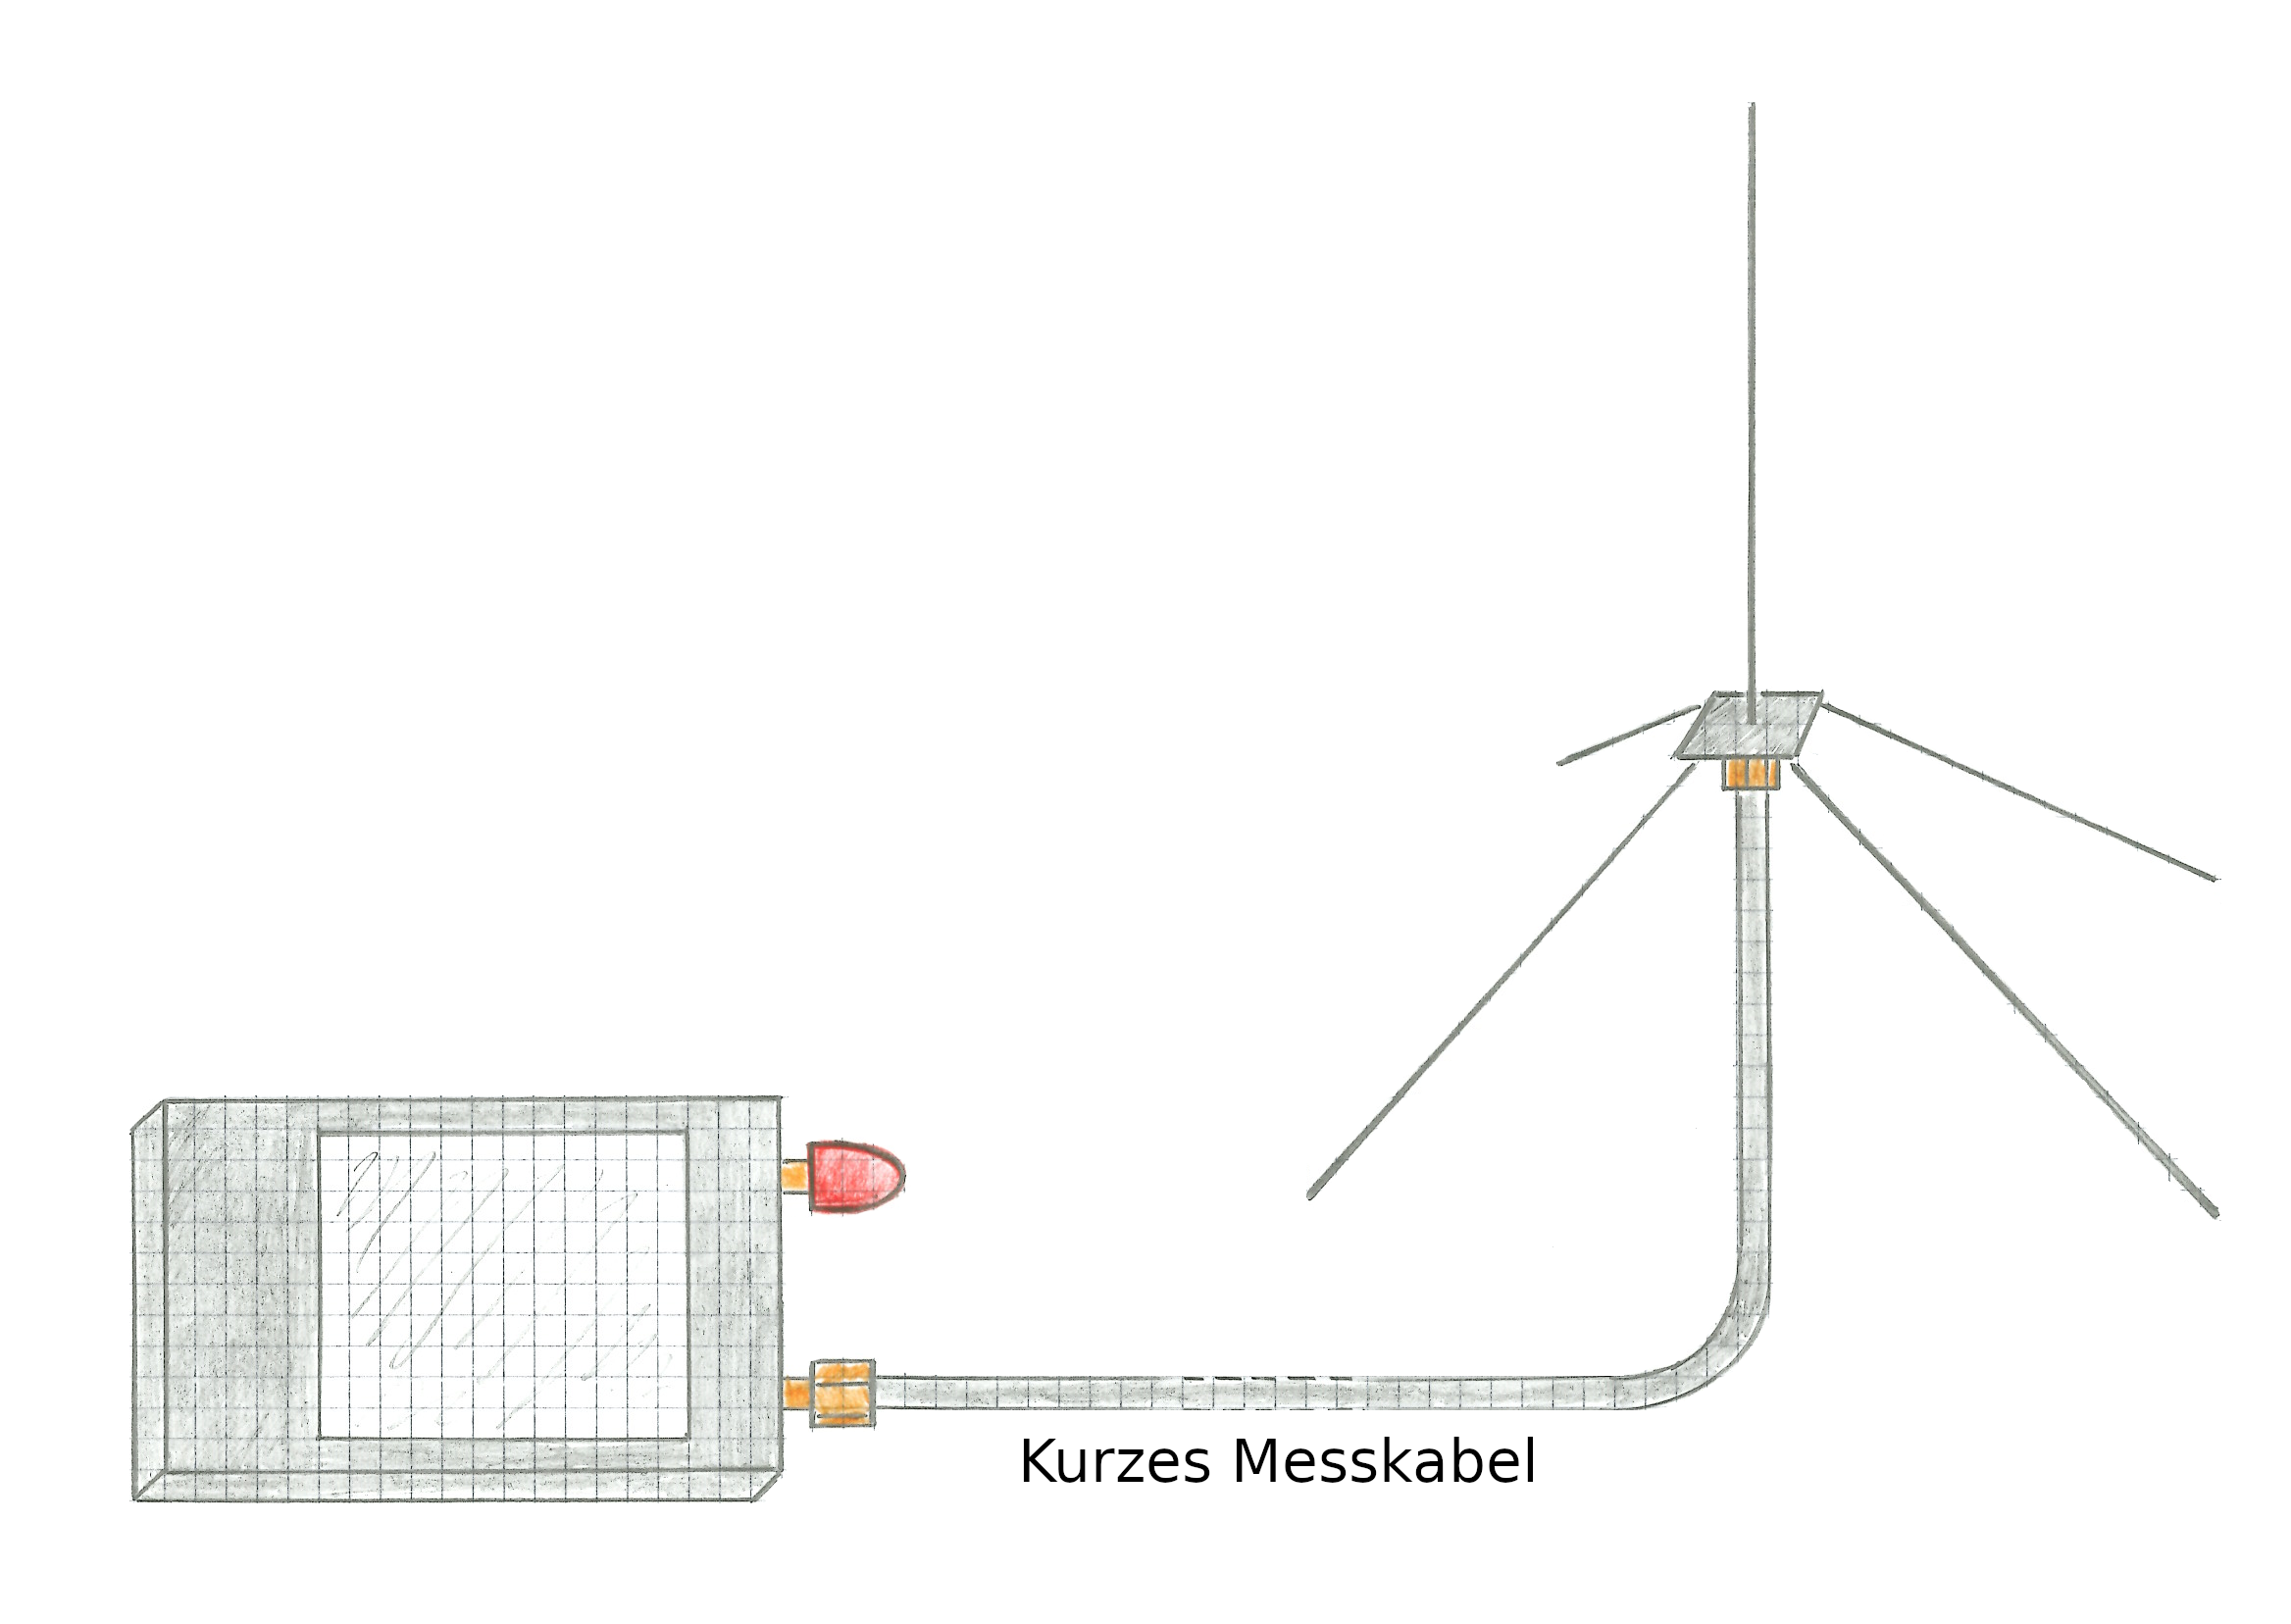
\includegraphics[width=\textwidth]{figures/illustration_antenna.png}
    \caption{Illustration der Charakterisierung einer Antenne mit einem kurzen Messkabel. Die Kalibrierung erfolgt am Fusspunkt.}
    \label{fig:antennenmessung}
\end{figure}

\newpage % FIXME
\section{Impedanzmessungen}\label{sec:impedance}
Der NanoVNA kann die Impedanz von Widerständen, Spulen, Kondensatoren, Abschlüssen etc.
bestimmen, da er in der Lage ist, sowohl Amplitude, wie auch Phasenverschiebung zu
quantifizieren. Im Gegensatz zu einem LCR-Meter kann der VNA auf der Frequenz messen,
auf der das Bauteil schlussendlich betrieben wird. Es wäre beispielsweise denkbar,
dass Streukapazitäten zwischen den Windungen einer Spule auf dieser Betriebsfrequenz
nicht mehr vernachlässigbar sind. Was im LCR-Meter bei einigen 100~kHz nach einer
ausgezeichneten Spule aussieht, wird dann bei höheren Frequenzen zu einem Schwingkreis
und erfüllt seinen Zweck nicht mehr.

Mit seiner Quell-Impedanz von 50~\Ohm bildet entsteht bei einer
Reflexionsmessung der Spannungsteiler aus Abbildung
\ref{fig:phasenverschiebung}. So kann das Gerät die Impedanz des Prüflings
berechnen und, unter Zuhilfenahme der momentanen Frequenz des Stimulus, bei
Bedarf daraus sogar die Induktivität bzw. Kapazität berechnen.

Es gibt drei gängige Wege, die Impedanz $Z$ eine Bauteils mit einem VNA zu messen:
(1) Eine Reflexionsmessung, (2) eine Transmissionsmessung mit der unbekannten
Impedanz in Serie, und (3) eine Transmissionsmessung mit der unbekannten
Impedanz parallel zu den Ports. Diese drei Varianten sind in Abbildung
\ref{fig:impedancemeasurement} gezeigt. Falls eine genaue Messung gewünscht ist,
kann ein unbekanntes $L$ mit einem bekannten Referenz-$C$ in Serie geschaltet
und die Resonanzfrequenz des so entstandenen Schwingkreises ermittelt werden.
Aus dieser Resonanzfrequenz kann anschliessend das unbekannte $L$ berechnet werden.
Diese Methode ist genauer als die anderen drei Ansätze -- bei einem unbekannten
$C$ würde analog ein bekanntes Referenz-$L$ verwendet werden.

\begin{figure}[H]
    \scalebox{0.8}{
    \begin{circuitikz} \draw
        (0.5,0) to[short,o-] (1,0) to[short] (3,0)
        (3,0) to[L=$Z$] (3,-2) to[short,-o] (0.5,-2);
        \node at (0.5,-1) {\small{Port 1}};
        \node at (2,-2.5) {\small{(1)}};
     \end{circuitikz}}
    \hfill
    \scalebox{0.8}{
    \begin{circuitikz} \draw
        (0.5,0) to[short,o-] (1,0) to[L=$Z$] (3,0) to[short,-o] (3.5,0)
        (0.5,-2) to[short,o-o] (3.5,-2);
        \node at (0.5,-1) {\small{Port 1}};
        \node at (3.5,-1) {\small{Port 2}};
        \node at (2,-2.5) {\small{(2)}};
     \end{circuitikz}}
    \hfill
    \scalebox{0.8}{
    \begin{circuitikz} \draw
        (0.5,0) to[short,o-o] (3.5,0)
        (0.5,-2) to[short,o-o] (3.5,-2)
        (2,0) to[L=$Z$,*-*]  (2,-2);
        \node at (0.5,-1) {\small{Port 1}};
        \node at (3.5,-1) {\small{Port 2}};
        \node at (2,-2.5) {\small{(3)}};
     \end{circuitikz}}
     \caption{Drei Varianten zur Messung einer Unbekannten Impedanz $Z$. Von
         links nach rechts: (1) Reflexionsmessung, (2) Transmissionsmessung mit $Z$ in
     Serie, (3) Transmissionsmessung mit $Z$ parallel zu den Ports.}
    \label{fig:impedancemeasurement}
\end{figure}

Gemäss \cite{tech2018performing} ist Variante (1), also die Reflexionsmessung, generell
empfohlen. Bei sehr grossen Impedanzen führt Variante (2), also Transmissionsmessung
mit $Z$ in Serie, zu genaueren Resultaten, und bei sehr kleinen Impedanzen
ist Variante (3), also Transmissionsmessung mit parallelem $Z$, zu bevorzugen.

Für eine genaue Messung muss das zu charakterisierende Bauteil in eine Test-Vorrichtung
(engl. test fixture) montiert werden. Die Qualität der Messung ist dabei vielfach
mehr abhängig von der Qualität dieser Vorrichtung als von derjenigen des verwendeten
Messgerätes. Der Anspruch an die Vorrichtung steigt mit zunehmender Frequenz,
denn kleine parasitäre Komponenten gewinnen dann an Einfluss. Abbildung
\ref{fig:testfixtures} zeigt verschiedene Ansätze für solche Vorrichtungen.
Oben links wurde aus SMA-Steckern und Krokodilklemmen eine vielseitig
einsetzbare Apparatur gebaut. Insbesondere bei höheren Frequenzen ist dieser
Ansatz jedoch völlig ungenügend. Oben rechts ist eine bessere Alternative zu
sehen: Auf eine freiliegende 50~\Ohm Leiterbahn kann dort das unbekannte
Bauteil aufgelötet werden. Besonders raffiniert ist der Aufbau von Larry
Benko), der aus Koaxialbuchsen einfach gebaut werden kann
\cite{benko2020impedance}.  Wie im unteren Teil von Abbildung
\ref{fig:testfixtures} zu sehen, kann ein Bauteil zwischen zwei rechtwinklig
zueinander liegenden N-Buchsen auf die drei oben genannten Arten (A-C für (1),
A-B für (2) und AB-C für (3)) montiert werden.

\minisec{Vorgehen mit dem NanoVNA (Reflexionsmessung, Variante (1)):}

\begin{enumerate}
    \item Test-Vorrichtung befestigen (z.B. Klemmen).
    \item Frequenzbereich einstellen.
    \item Kalibrierung für Reflexionsmessung: Klemmen kurzschliessen für Kurzschluss, 50 Ohm Widerstand
        einsetzen für Last.
    \item Bauteil in Vorrichtung einsetzen (Abbildung \ref{fig:illustrationimpedance})
    \item Anzeigeformat (``Display'' $\longrightarrow$ ``Format''): Smith.
    \item Kanalwahl (``Display'' $\longrightarrow$ ``Channel''): CH0 (Reflexionsmessung).
    \item Marker verwenden und Werte ablesen.
\end{enumerate}

\begin{figure}[H]
    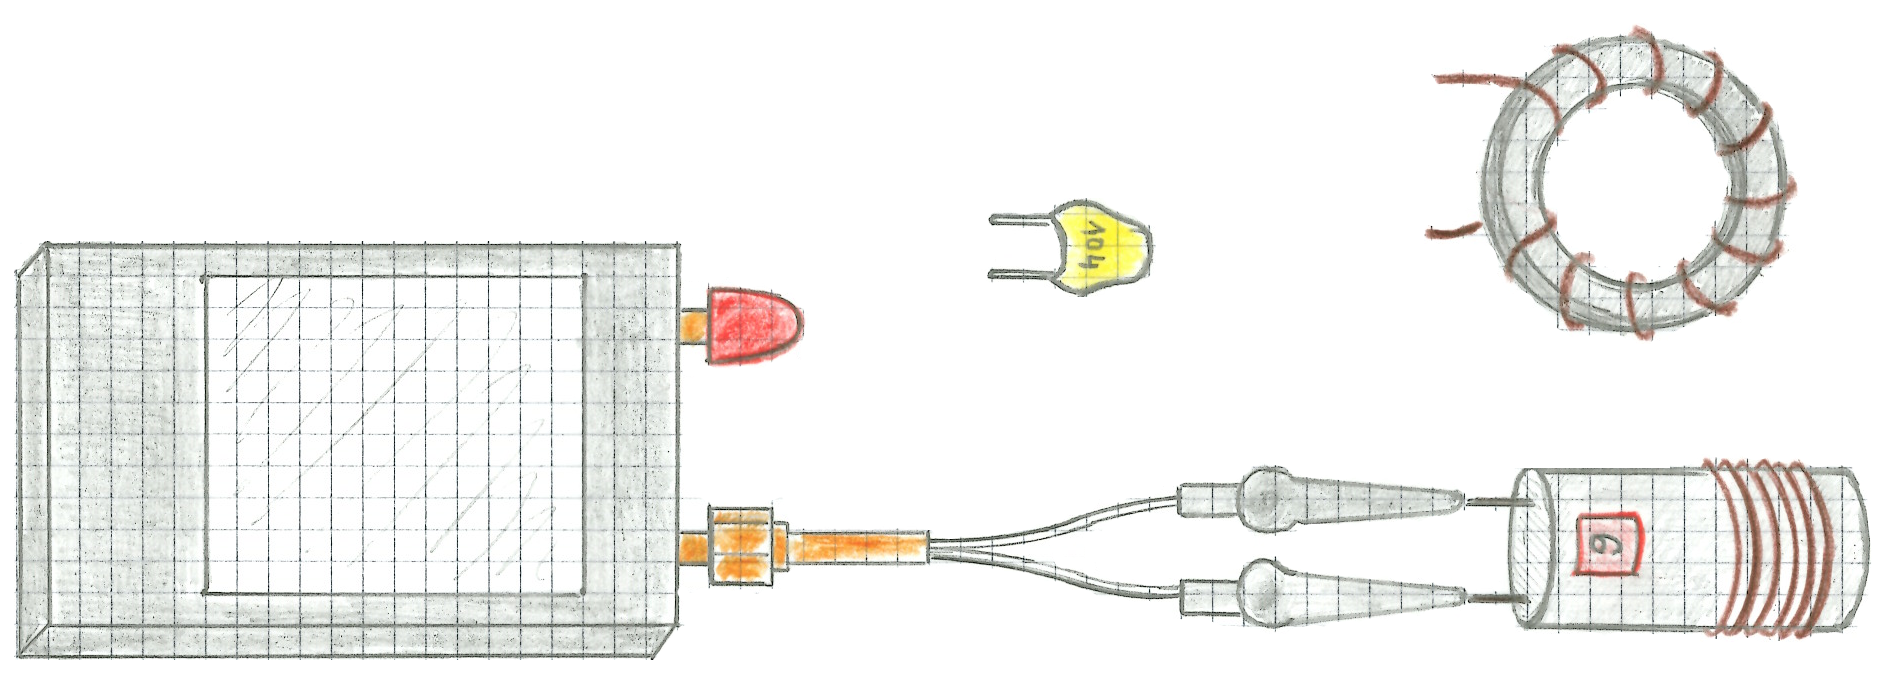
\includegraphics[width=\textwidth]{figures/illustration_impedance.png}
    \caption{Illustration der Charakterisierung einer Antenne mit einem kurzen Messkabel. Die Kalibrierung erfolgt am Fusspunkt.}
    \label{fig:illustrationimpedance}
\end{figure}

\begin{figure}\begin{center}
    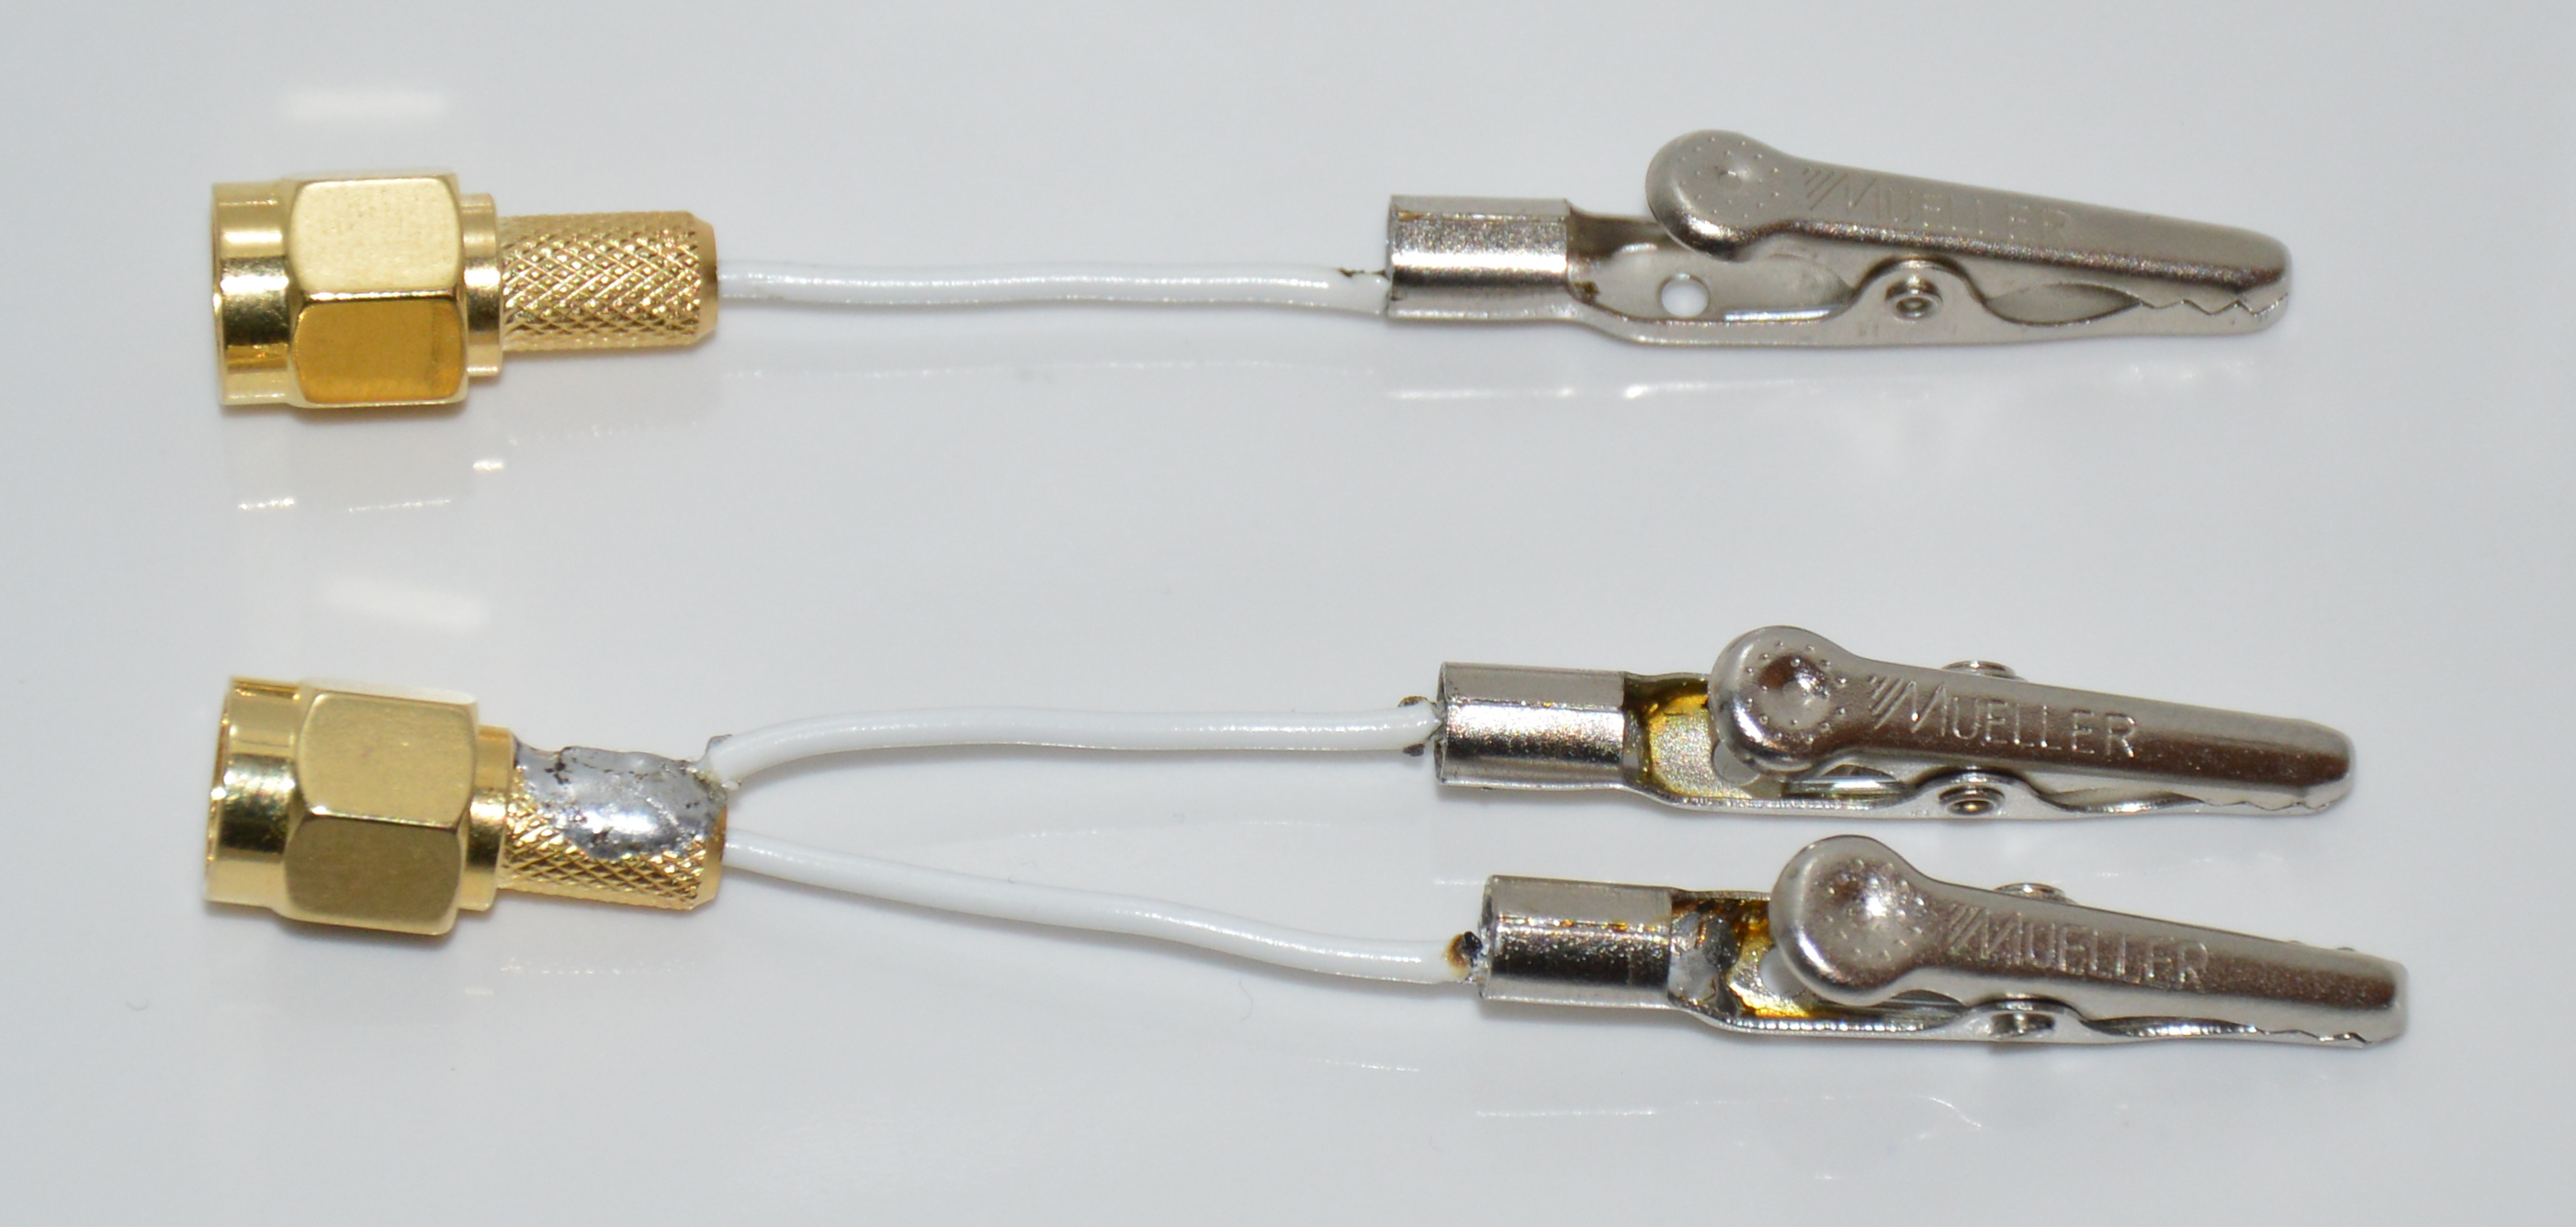
\includegraphics[height=36mm]{figures/klemmen.jpg}\hfill
    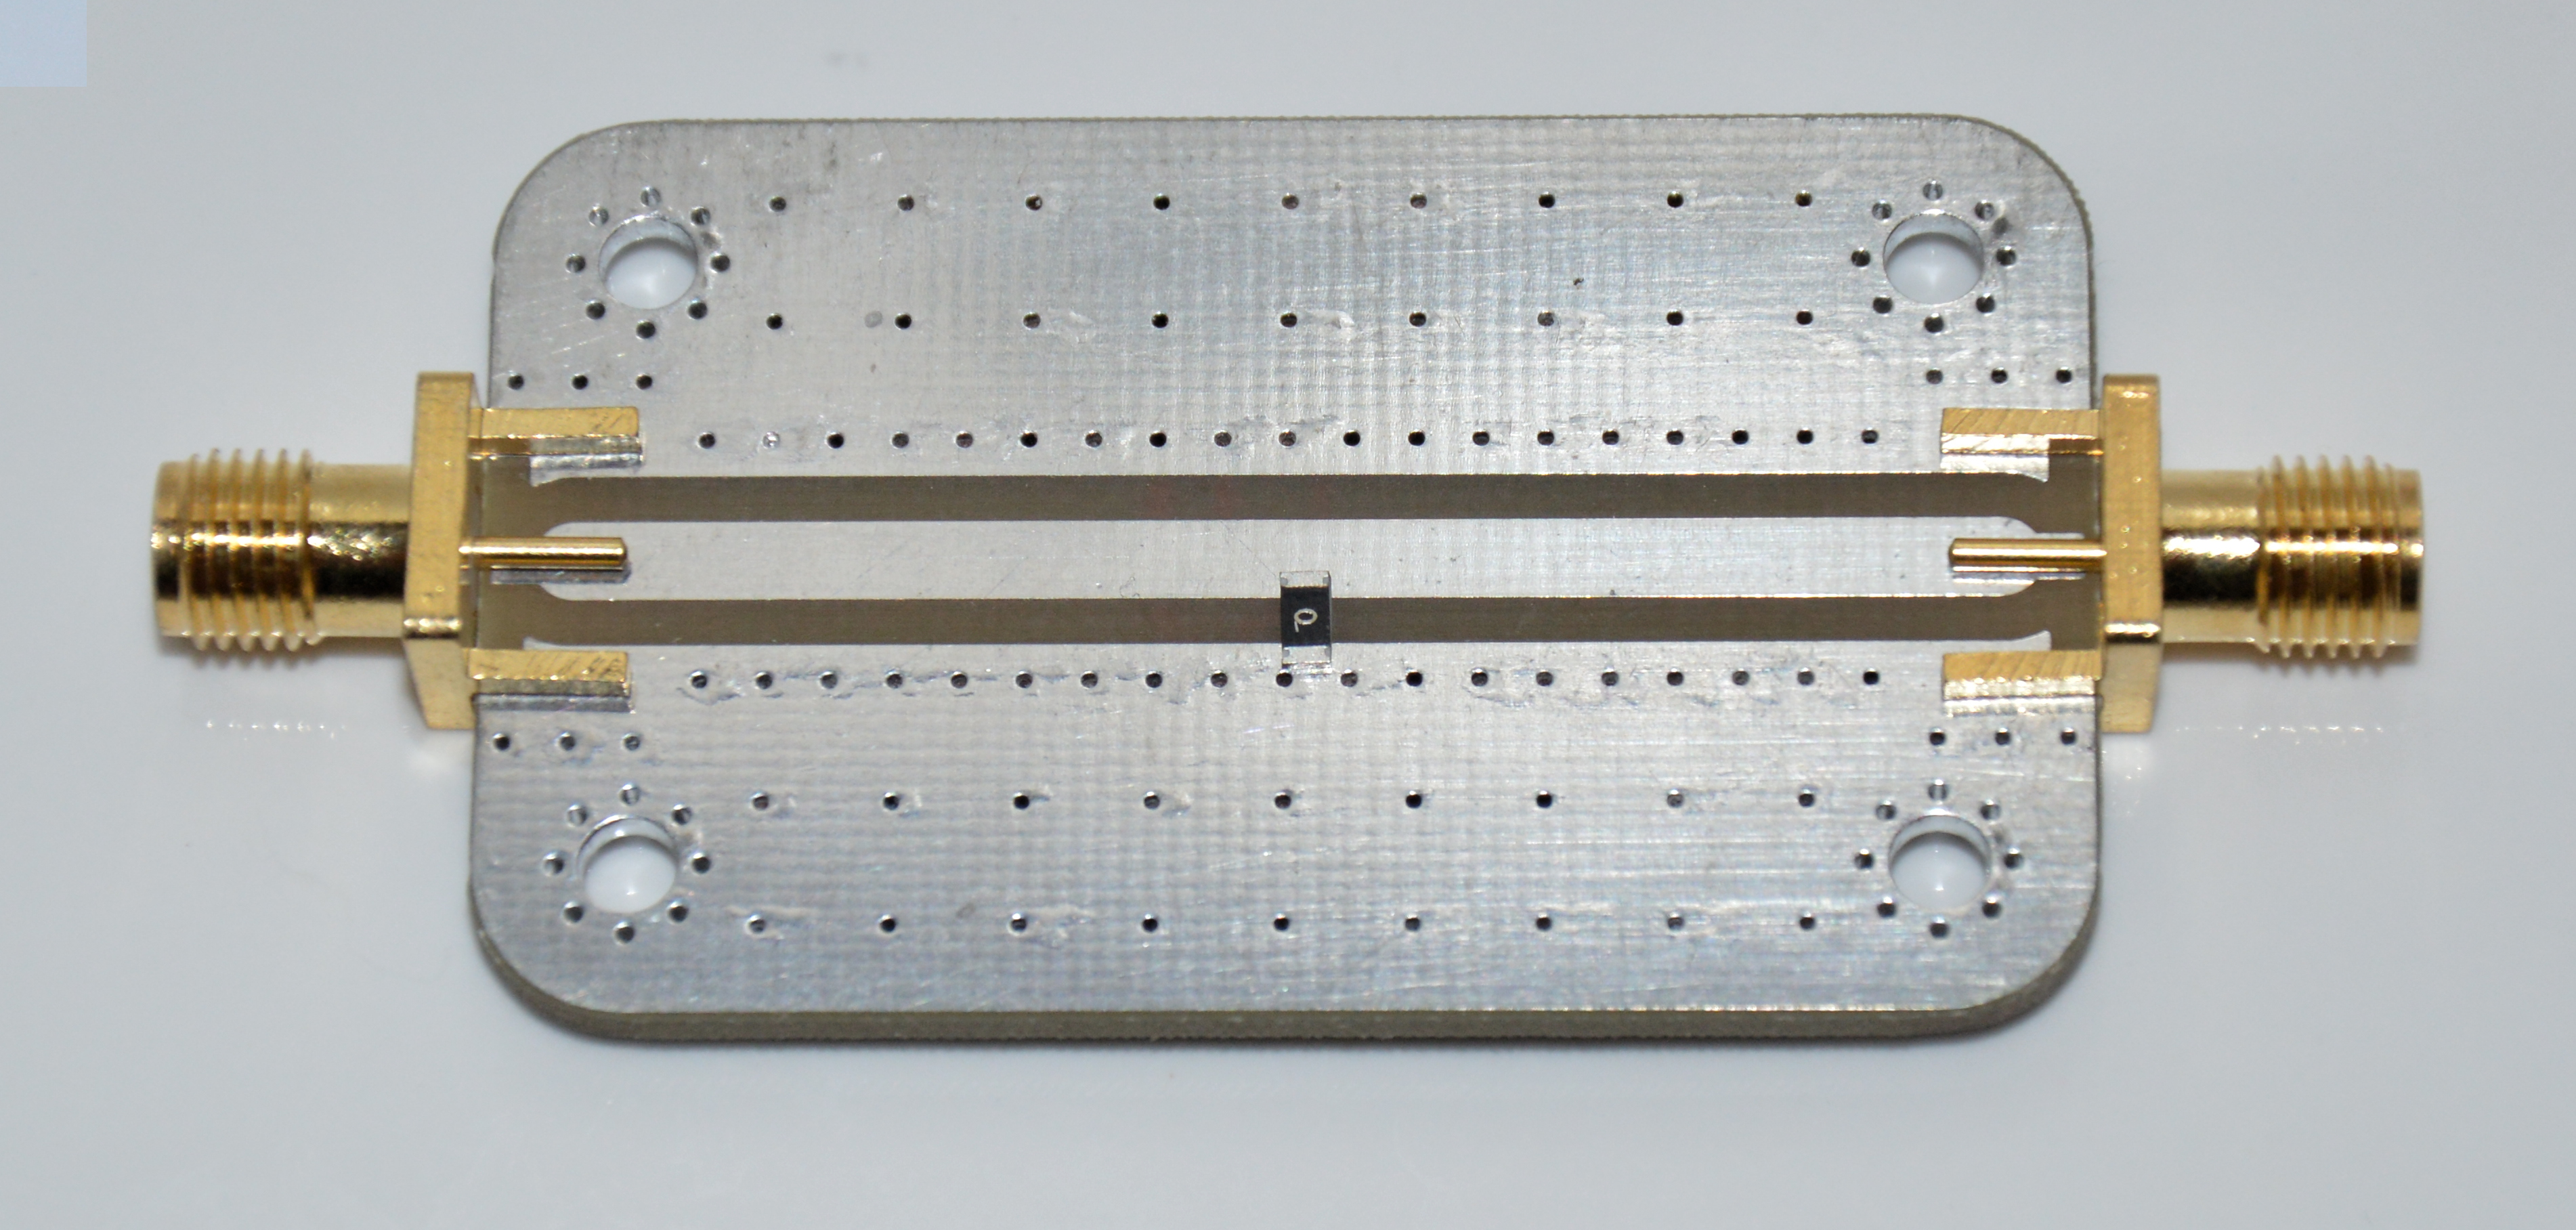
\includegraphics[height=36mm]{figures/impedanzpcb.jpg}

    \includegraphics[width=\textwidth]{figures/w0qe_fixture.png}
    \caption{Oben links: Klemmen zur Impedanzmessung. Oben rechts: Leiterplatte zur Impedanzmessung
        mit 50~\Ohm Spur und eingesetztem Bauteil gemäss Messvariante (3). Unten: Vorrichtung von Larry Benko zur Impedanzmessung mit einem VNA \cite{benko2020impedance}.
    Ein zu charakterisierendes Bauteil wird gemäss einer der drei Varianten aus Abbildung \ref{fig:impedancemeasurement}
    an die Koaxialbuchsen gelötet.}
    \label{fig:testfixtures}
\end{center}\end{figure}

\newpage % FIXME
\section{Schwingkreise, Resonanzfrequenzen, Anpassung}\label{sec:schwingkreis}
Es gibt mehrere Gründe, sich mit der Messung von Schwingkreisen
auseinanderzusetzen. Der einfachste besteht darin, die Resonanzfrequenz
eines solchen zu ermitteln -- dies schliesst auch die Eigenresonanzfrequenz von
Bauteilen ein. Dann ist es möglich, Spulen und Kondensatoren genauer zu
bestimmen, indem sie zu einem Schwingkreis geschaltet werden: Ist die
Induktivität einer Spule gesucht, wird diese Spule mit einem Kondensator
mit bekannter Kapazität zu einem Schwingkreis verschaltet, die Resonanzfrequenz
gemessen und mit der gemessenen Resonanzfrequenz $f$ und der bekannten
Kapazität $C$ die gesuchte Induktivität $L$ berechnet. Schliesslich sind
Schwingkreise einfache Modelle von Antennen.

\subsection{Schwingkreis und Resonanzfrequenz}
Ein Schwinkreis ergibt sich, wenn ein Widerstand $R$, eine Induktivität $L$
und eine Kapazität $C$ in Serie geschaltet werden (Serienschwingkreis, siehe
Abbildung \ref{fig:schwingkreis}). Es besteht auch die Möglichkeit, diese drei
Bauteile parallel zu schalten (Parallelschwingkreis).

\begin{figure}[H]
    \begin{center}
    \begin{circuitikz} \draw
        (0,0) to[short,o-] (1,0) to[L=$L$] (3,0) to[C=$C$] (5,0) to[R=$R$] (7,0) to[short,-o] (8,0);
    \end{circuitikz}
    \end{center}
    \caption{Ein Serienschwingkreis bestehend aus einer Spule/Induktivität $L$,
    einem Kondensator/Kapazität $C$ und einem Widerstand $R$.}
    \label{fig:schwingkreis}
\end{figure}

Bei einer bestimmten Frequenz, der Resonanzfrequenz $f_r$, heben sich die
Blindwiderstände von $L$ und $C$ genau auf. Es gilt:

$$
f_r = \frac{1}{2\pi\sqrt{L\cdot C}}
$$

Sind also $L$ und $C$ bekannt, so lässt sich $f_r$ berechnen, ebenso lässt ich
$L$ berechnen, falls $C$ und $f_r$ bekannt sind, etc. Abbildung \ref{fig:resonanzplot}
zeigt den Blindwiderstand (links, gestrichelte Linie) im Serienschwingkreis als Funktion der Frequenz. Es
handelt sich dabei um die Darstellung der Grösse $X_L-X_C$ aus Abbildung \ref{fig:XRLC}.
Unterhalb der Resonanzfrequenz ist der Blindwiderstand negativ, der
Schwingkreis hat also eine kapazitive Komponente bzw. der Kondensator
dominiert. Oberhalb der Resonanzfrequenz ist der Blindwiderstand positiv, der
Schwingkreis ist induktiv bzw. die Spule dominiert. Bei einer Resonanzfrequenz
von $f_r\approx$~5~MHz ist der Blindwiderstand 0~$\Omega$, lediglich $R=50$~$\Omega$
ist am Eingang sichtbar. Ein Abschluss von 50~$\Omega$ entspricht einer perfekten
Anpassung und deshalb entsteht bei dieser Frequenz überhaupt kein Rückfluss.
Die selben Sachverhalte sind auf der rechten Seite von Abbildung
\ref{fig:resonanzplot} im Smith-Diagram erkennbar. Die Analogie zu Verhalten
einer Antenne im Umfeld ihrer Resonanzfrequenz ist offensichtlich.
\begin{figure}
\begin{center}\begin{tikzpicture}
\begin{axis}[
    xmin=1, xmax=9,
    ymin=-70,ymax=10,
    grid=both,
    xlabel={Frequenz $f$/MHz},
    ylabel={\uline{R\"uckfluss}},
    height=6cm,
    width=0.45\textwidth,
    major grid style={black!10}
]
\addplot[mark=none,color=HB9UFblue,thick]  table[x index = {0}, y index = {1}] {schwingkreis.dat};
\end{axis}
\begin{axis}[
    xmin=1, xmax=9,
    ymin=-280,ymax=40,
    grid=none,
    separate axis lines,
    ylabel style = {align=center},
    ylabel={\udash{Blindwiderstand $X/\Omega$}},
    ticks=none,
    xmajorticks=false,
    xminorticks=false,
    ymajorticks=true,
    yminorticks=false,
    scaled ticks=false,
    ytick = {-240,-160,-80,0},
    axis y line*=right,
    height=6cm,
    width=0.45\textwidth,
    major grid style={black!10}
]
\addplot[mark=none,dashed,color=HB9UFred,thick]  table[x index = {0}, y index = {2}] {schwingkreis.dat};
\fill [fill=black] (axis cs:5.033,0) circle [radius=2pt];
\node [below]  at  (axis cs:5.033,0) {$f_r$};
\end{axis}
\end{tikzpicture}
\hfill
\begin{tikzpicture}
    \begin{smithchart}[width=0.46\textwidth]
\pgfplotsset{yticklabel in circle}
\addplot[thick,smooth,color=HB9UFblue] table[x index = {3}, y index = {4}] {schwingkreis.dat};
\fill [fill=black] (axis cs:1,0) circle [radius=2pt];
\node [below left]  at  (axis cs:1,0) {$f_r$};
\end{smithchart}
\end{tikzpicture}\end{center}
\caption{Links: Rückfluss und Blindwiderstand des Schwingkreises aus Abbildung \ref{fig:schwingkreis} mit 
$L$=1~$\mu$H, $C$=1~nF, $R$=50~$\Omega$. Rechts: Smith-Diagramm der Eingangsimpedanz dieser Schaltung.}
\label{fig:resonanzplot}
\end{figure}

\subsection{Anpassung}
Manchmal ist es wünschenswert, eine Impedanz in eine andere umzuwandeln. Dies ist beispielsweise der Fall,
wenn ein hochomiges Bauteil in einem 50~$\Omega$ System verwendet werden soll, oder wenn eine Last
(z.B. Antenne) auf der Zielfrequenz eine Impedanz aufweist, die fernab der Systemimpedanz liegt und eine
genügende Leistungsübertragung nicht erbracht wird. In diesem Fall kommen Transformatoren zur Impedanzwandlung
(siehe Abschnitt \ref{sec:impedanztrafo}), speziell konfigurierte Leitungen
oder Anpass-Netzwerke zum Einsatz. Letztere bestehen aus Kombinationen von Kapazitäten und Induktivitäten,
mit denen die Impedanzanpassung vorgenommen wird. Die einfachste Möglichkeit hierfür ist der in Abbildung
\ref{fig:lmatch} gezeigte L-Match.

\begin{figure}[H]
    \scalebox{0.8}{
    \begin{circuitikz} \draw
        (0.5,0) to[short,o-] (1,0) to[C] (3,0) to[short,-o] (3.5,0)
                             (3,0) to[L,*-] (3,-2) node[ground] {};
     \end{circuitikz}}
    \hfill
    \scalebox{0.8}{
    \begin{circuitikz} \draw
        (0.5,0) to[short,o-] (1,0) to[L] (3,0) to[short,-o] (3.5,0)
                             (3,0) to[C,*-] (3,-2) node[ground] {};
     \end{circuitikz}}
    \hfill
    \scalebox{0.8}{
    \begin{circuitikz} \draw
        (0.5,0) to[short,o-] (1,0) to[L] (3,0) to[short,-o] (3.5,0)
                             (3,0) to[L,*-] (3,-2) node[ground] {};
     \end{circuitikz}}
    \hfill
    \scalebox{0.8}{
    \begin{circuitikz} \draw
        (0.5,0) to[short,o-] (1,0) to[C] (3,0) to[short,-o] (3.5,0)
                             (3,0) to[C,*-] (3,-2) node[ground] {};
    \end{circuitikz}}

    \vspace{3em}
    % zweite Reihe startet hier
    \scalebox{0.8}{
    \begin{circuitikz} \draw
        (0.5,0) to[short,o-] (1,0) to[C] (3,0) to[short,-o] (3.5,0)
                             (1,0) to[L,*-] (1,-2) node[ground] {};
     \end{circuitikz}}
    \hfill
    \scalebox{0.8}{
    \begin{circuitikz} \draw
        (0.5,0) to[short,o-] (1,0) to[L] (3,0) to[short,-o] (3.5,0)
                             (1,0) to[C,*-] (1,-2) node[ground] {};
     \end{circuitikz}}
    \hfill
    \scalebox{0.8}{
    \begin{circuitikz} \draw
        (0.5,0) to[short,o-] (1,0) to[L] (3,0) to[short,-o] (3.5,0)
                             (1,0) to[L,*-] (1,-2) node[ground] {};
     \end{circuitikz}}
    \hfill
    \scalebox{0.8}{
    \begin{circuitikz} \draw
        (0.5,0) to[short,o-] (1,0) to[C] (3,0) to[short,-o] (3.5,0)
                             (1,0) to[C,*-] (1,-2) node[ground] {};
    \end{circuitikz}}

    \caption{L-Match: Verschiedene Anordnungen von Kapazitäten und Induktivitäten zur Anpassung der Impedanz.}
    \label{fig:lmatch}
\end{figure}

Keine dieser Schaltungen ermöglicht die Anpassung einer beliebigen Impedanz zu
einer anderen beliebigen Impedanz. Es ist allerdings möglich, die Bauteilwerte
variabel zu gestalten und mehrere L-Matches zusammenzuschalten, um die
Anpassungemöglichkeiten zu erweiterten. Ein in diesem Sinn beliebter Ansatz 
ist der in Abbildung \ref{fig:tmatch} dargestellte T-Match.

\begin{figure}[H]
    \begin{center}
    \begin{circuitikz} \draw
        (0,0) to[short,o-] (1,0) to[vC,mirror] (3,0) to[vC,mirror] (5,0) to[short,-o] (6,0)
        (3,0) to[short,*-] (3,-1) to[vL,invert,mirror] (3,-3) node[ground] {};
    \end{circuitikz}
    \end{center}
    \caption{T-Match: Beliebte Schaltung zur Impedanzanpassung (Matchbox/Antennen-Tuner). Es handelt sich um einen
    Verbund zweier variabler L-Matches aus Abbildung \ref{fig:lmatch}.}
    \label{fig:tmatch}
\end{figure}

\minisec{Vorgehen mit dem NanoVNA:}

Die Messung Schwingkreis-Verhaltens wird genau gleich durchgeführt wie die
Impedanzmessung in Abschnitt \ref{sec:impedance} (Reflexionsmessung). Statt
eines einzelnen Bauteils wird der ganze Schwingkreis angeschlossen.

\newpage % FIXME
\section{Filter, Dämpfungsglieder, Koppler und Ähnliches}\label{sec:filter}
Filter lassen einige Frequenzen des Spektrums passieren (Passband), während
sie andere Frequenzen reflektieren oder dissipieren. Die Pass- und
Sperr-Charakteristika von Filtern werden üblicherweise mit einer
Transmissionsmessung bestimmt. Unter Umständen ist allerdings auch eine
Reflexionsmessung zielführend, z.B. wenn ein Duplexer justiert werden muss.
Handelt es sich bei dem Filter nicht um ein 50~$\Omega$ System (z.B. ein
Keramik-Filter), muss die Fehlanpassung berücksichtigt werden.

Zu beachten ist wie üblich, dass keine Einfügedämpfungen gemessen werden
können, welche den Dynamikbereich des VNAs überschreiten.

\subsection{Koaxiale Stub-Filter}\label{sec:stubfilter}
Eine Leitung -- z.B. ein Koaxialkabel -- der Länge $\lambda/4$ hat besondere
Eigenschaften: Ein Kurzschluss am einen Ende sieht vom anderen Ende aus wie
eine offene Verbindung; eine offene Verbindung am einen Ende sieht vom anderen
Ende aus wie ein Kurzschluss. Die Impedanz wird also transformiert, die
Struktur wird deshalb auch Viertelwellentransformator genannt. Im Smith-Diagramm
wird eine Abschlussimpedanz am Ende der Leitung in einem Halbkreis im Gegenuhrzeigersinn
rotiert. Zwei $\lambda/4$-Leitungen hintereinander entsprechen einer Leitung
der Länge $\lambda/2$, im Smith-Diagramm erfolgen zwei Rotationen um je einen
Halbkreis bzw. eine Rotation um einen Vollkreis: Die $\lambda/2$-Leitung
transformiert eine beliebige Impedanz (abgesehen von Verlusten im Kabel) auf
sich selbst.

\begin{figure}[H]
\begin{center}
\begin{tikzpicture}
\begin{axis}[
    xmin=0, xmax=300,
    ymin=-35, ymax=5,
    grid=both,
    xlabel={Frequenz / MHz},
    ylabel={Transmission / dB},
    xtick = {0,30,...,300},
%   ticks=none,
    height=6cm,
    width=0.9\textwidth,
    major grid style={black!10}
]
\addplot[color=HB9UFblue,thick] table[,x index = {0}, y index = {1}] {quarterwave.dat};
\addplot[color=HB9UFred,thick,dashed] table[,x index = {0}, y index = {2}] {quarterwave.dat};
\end{axis}
\end{tikzpicture}
\end{center}
\caption{Einfügedämpfung eines Stub-Filters der Länge 2.5~m. Die ausgezogene Linie beschreibt den Filterverlauf
eines kurzgeschlossenen Stubs, wärend die gestrichelte Linie den Filterverlauf eines Stubs mit offenem Ende beschreibt.}
\label{fig:quarterwaveplot}
\end{figure}

Diese Eigenschaft kann genutzt werden, um mit Koaxialkabel einen relativ
schmalbandigen Sperr-Filter (Notch) zu implementieren (siehe Abbildung
\ref{fig:quarterwaveplot}). Dazu wird, wie in Abbildung
\ref{fig:quarterwavestub} gezeigt, mit einem T-Stück die $\lambda/4$-Leitung
parallel geschaltet. Als Alternative zum T-Stück kann auch eine Vorrichtung wie
die Platine in Abbildung \ref{fig:testfixtures} genutzt werden -- dies ist vor
allem dann sinnvoll, wenn die $\lambda/4$-Leitung ohne Stecker auskommen soll.

Die Viertelwellentransformation mag etwas verwirrend erscheinen, ein Zahlenbeispiel
soll deshalb an dieser Stelle für etwas Klarheit sorgen: Für eine Frequenz von
30~MHz ist die Wellenlänge ca. $\lambda$=10~m. Eine Halbwellenleitung hat deshalb
die Länge $\lambda/2$=5~m und eine Vierteilwellenleitung $\lambda/4$=2.5~m. Ein
Kurzschluss am Ende dieser $\lambda/4$ Leitung wird deshalb bei 30~MHz zu einer
offenen Verbindung transformiert, welche die beiden anderen am T-Stück
angeschlossenen Leitungen keinen Einfluss hat. Bei der doppelten Frequenz, also
60~MHz, hat diese Leitung aber nicht mehr die Länge  $\lambda/4$, sondern
$\lambda/2$! Da die Leitung am Ende nach wie vor kurzgeschlossen ist, wird dieser
Kurzschluss bei 60~MHz also unmittelbar in das T-Stück transformiert, und ein
Kurzschluss führt zu einer Totalreflexion: Die Struktur sperrt bei 60~MHz. Das
selbe Phänomen tritt auch bei 120~MHz, 180~MHz etc. auf. Die Einfügedämpfung
ist in Abbildung \ref{fig:quarterwaveplot} dargestellt. Die gestrichelte Linie
zeigt ein Stub mit offenem (anstelle eines kurzgeschlossenen) Ende. Die Sperrwirkung
erfolgt dort bereits bei 30~MHz, da bei dieser Frequenz das offene Ende in einen
Kurzschluss transformiert wird.

\begin{figure}[t]
    \reflectbox{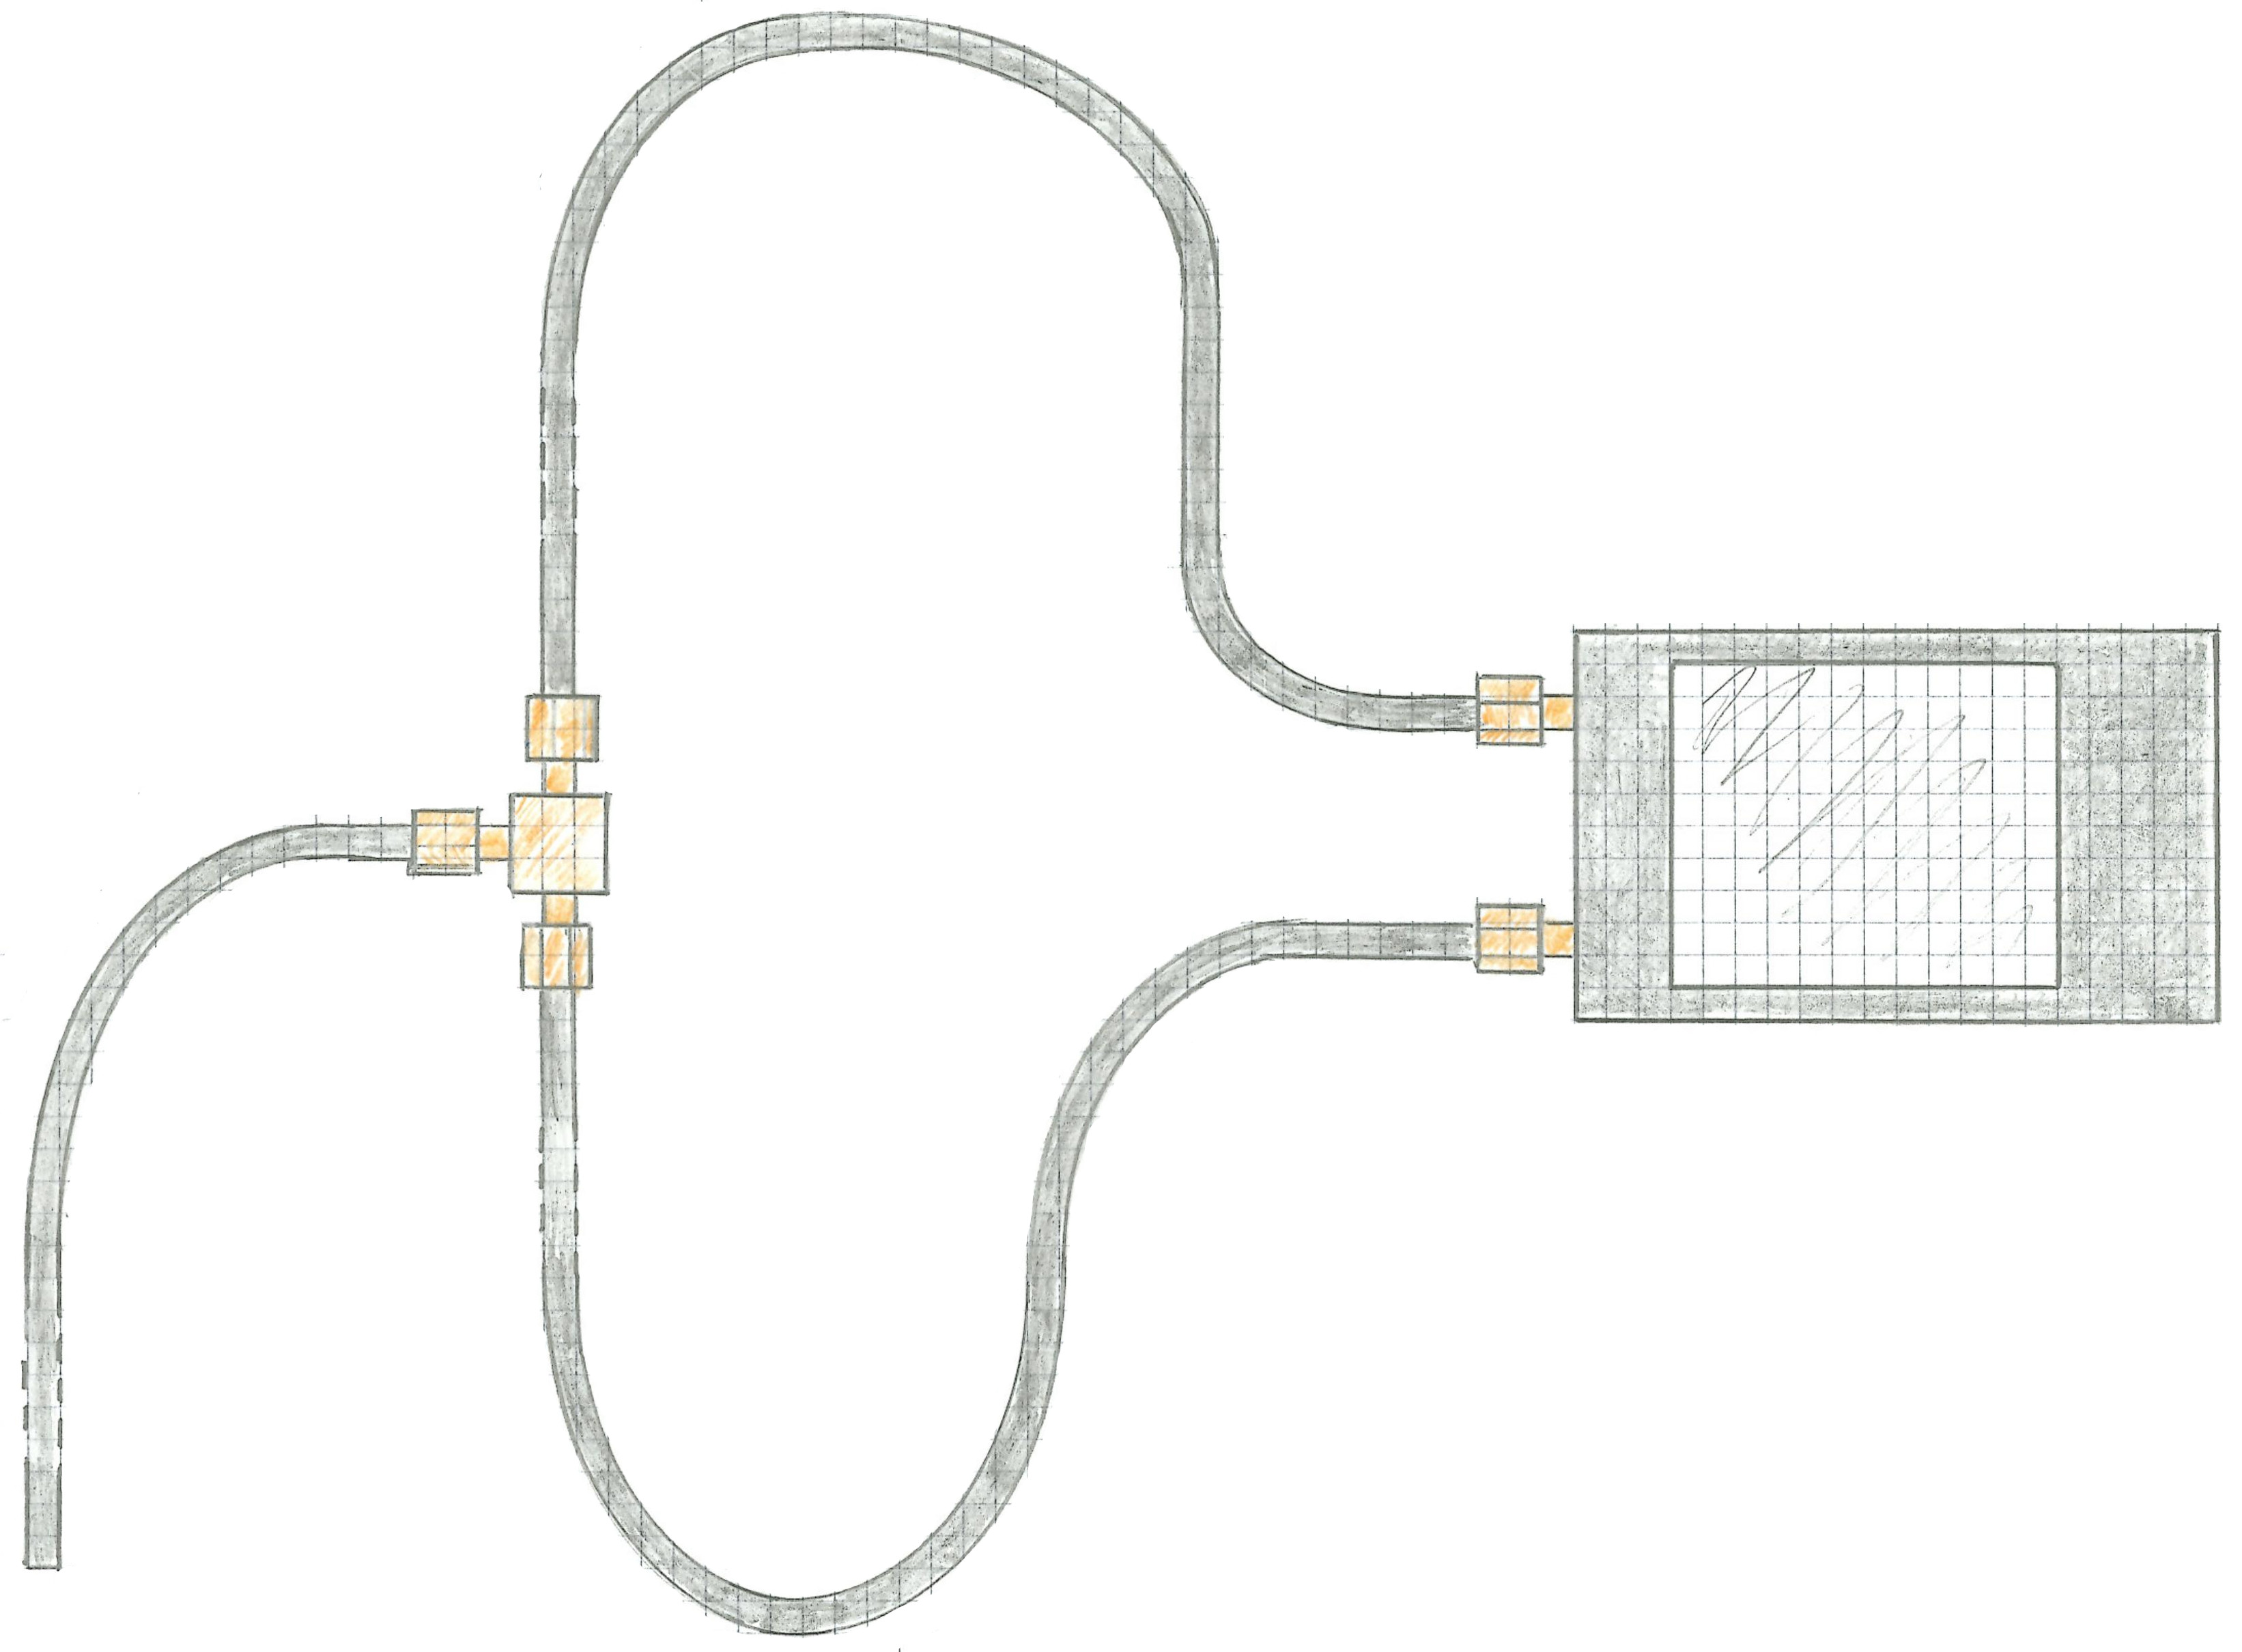
\includegraphics[width=\textwidth]{figures/illustration_stub.jpg}}
    \caption{Transmissions-Messung eines Stub-Filters. Das Ende des Stubs kann
    (je nach gewünschtem Verhalten) offen oder kurzgeschlossen sein.}
    \label{fig:quarterwavestub}
\end{figure}

Das Vorgehen für die Messung eines Stub-Filters mit dem NanoVNA unterscheidet
sich nicht von den übrigen Filtermessungen in diesem Abschnitt. Weil aber
interessante leitungstheoretische Aspekte eine Rolle spielen, werden diese
Stub-Filter hier separat behandelt.

\subsection{Dämpfungsglieder, Koppler und Isolation}
Die Dämpfung oder Isolation zwischen zwei Anschlüssen von Dämpfungsgliedern,
Stufendämpfungsgliedern, Splitter-Combinern, Richt-, Hybrid- und anderer Koppler
kann ebenfalls mit einer Transmissionsmessung ermittelt werden. Dazu wird der VNA auf den
gewünschten Frequenzbereich eingestellt, mit einem Verbindungsstück kalibriert
und dann eingeschleift. Damit unterschiedet sich diese Messung nicht von derjenigen
von Filtern.

Bei vollständiger Isolation wäre die Einfügedämpfung unendlich gross. Trotzdem
zeigt ein VNA einen endlichen Wert an. Wie bereits mehrfach erwähnt kann kann
keine Dämpfung/Isolation gemessen werden, welche diesen Wert übersteigt.

\minisec{Vorgehen mit dem NanoVNA:}
Für alle Messungen in diesem Abschnitt \ref{sec:filter} gilt folgendes Vorgehen:

\begin{enumerate}
    \item Frequenzbereich einstellen.
    \item Messkabel anschliessen und mit Thru-Adapter verbinden.
    \item Kalibrierung für Transmissionsmessung durchführen.
    \item Filter einschleifen.
    \item Anzeigeformat (``Display'' $\longrightarrow$ ``Format''): LogMag.
    \item Kanalwahl (``Display'' $\longrightarrow$ ``Channel''): CH1 (Transmissionsmessung).
\end{enumerate}

Je nach Situation kann eine zusätzliche Reflexionsmessung der Filterports zielführend sein.

\newpage % FIXME
\section{Mantelwellensperren}
Eine Mantelwelle ist eine elektromagnetische Welle, die sich auf dem Aussenleiter (Mantel) eines
Koaxialkabels ausbreitet. Dies ist in aller Regel aus verschiedenen Gründen
unterwünscht; um die Mantelwelle zu unterbinden, wird eine Mantelwellensperre
eingesetzt. Diese Mantelwellensperre soll für Gegentaktsignale wie das
Empfangssignal von der Antenne zum Empfänger und das Sendesignal vom Sender
zur Antenne durchlässig sein; für Gleichtaktsignale wie die Mantelwelle soll
die Mantelwellensperre nicht durchlässig sein.

Die Messung einer Mantewellensperre hat deshalb drei Aspekte:

\begin{enumerate}
    \item Durchlässigkeit von Gegentaktsignalen.
    \item Dämpfung von Gleichtaktsignalen.
    \item Verhalten unter Last (Erwärmung etc.)
\end{enumerate}

Mit einem VNA werden typischerweise nur die ersten beiden Aspekte erfasst,
Erwärmung unter Last kann z.B. mit einem Thermomenter, einer Wärmebildkamera
etc. erfasst werden und wird an dieser Stelle nicht besprochen.

\subsection{Gegentaktmessung}\label{sec:gegentaktmessung}

Die Gegentaktmessung ist einfach: Der VNA wird für eine Transmissionsmessung
kalibriert, die Sperre wird eingeschleift und die Einfüngungsdämpdung wird
gemessen. Eine gute Mantelwellensperre sollte bei dieser Messung eine geringe
Einfügedämpfung aufweisen.

\subsection{Gleichtaktmessung}

Für die Gleichtaktmessung wird die Mantelwellensperre auf eine besondere
Art und Weise mit dem VNA verbunden: Der Eingang wird mit dem Stimulus,
der Ausgang mit dem detektierenden Port verbunden. Allerdings werden die
beiden beiden Leiter der Leitung jeweils kurzgeschlossen und mit dem
Innenleiter der Ports verbunden; die beiden Aussenleiter der Ports werden
kurzgeschlossen. Wenn die so präparierte Mantewellensperre als diskretes
Bauteil betrachtet wird, so entspricht diese Messung der seriellen
Transmissionsmessung dieses Bauteils -- also Messvariante (2) aus
Abschnitt \ref{sec:impedance}. Eine gute Mantelwellensperre
sollte bei dieser Messung eine hohe Einfügedämpfung haben.

Für diese Messung ist eine Vorrichtung notwendig, um die Aussenleiter der
beiden VNA-Ports kurzschliesst. Die Mantelwellensperre kann dann über Klemmen
mit den beiden Innenleitern verbunden werden. (Siehe Abbildung
\ref{fig:illustration_choke} für eine Vorrichtung mit Klemmen).

\begin{figure}
    % FIXME
    \includegraphics[width=\textwidth,draft,height=6cm]{figures/illustration_choke.jpg}
    \caption{Gleichtaktmessung von Mantelwellensperren. Die Mantelwellensperre
        ist in Serie zwischen den beien Ports geschaltet. FIXME: Mantelwellensperre
    nach W2DU \cite{maxwell1983w2du}. FIXME: Mantelwellensperre nach DG0SA.}
    \label{fig:illustration_choke}
\end{figure}

\minisec{Vorgehen mit dem NanoVNA:}
\begin{enumerate}
    \item NanoVNA für Gegentaktmessung vorbereiten wie in Abschnitt \ref{sec:filter} beschrieben.
        (Frequenz einstellen, Kalibrierung für Transmissionsmessung mit Thru, Kanalwahl ``CH1'',
        Anzeigeformat ``LogMag''.)
    \item Mantelwellensperre einschleifen, d.h. wie im normalen Gebrauch anschliessen.
    \item NanoVNA für Gleichtaktmessung vorbereiten: Messvorrrichtung montieren und für
        Transmissionsmessung rekalibrierung -- die Thru-Kalibrierung erfolgt mit kurzgeschlossener
        Vorrichtung.
    \item Dann Gleichtaktmessung wie in Abbildung \ref{fig:illustration_choke} durchführen.
\end{enumerate}

\newpage % FIXME
\section{Schwingquarz}
Ein Schwingquarz ist ein Bauteil, welches zur Erzeugung von Schwingungen oder
als Filter verwendet werden kann. Ein vereinfachtes Ersatzschaltbild ist in
Abbildung \ref{fig:quarzersatz} dargestellt. 

\begin{figure}[H]
    \begin{center}
    \begin{circuitikz} \draw
        (0,0) to[short,o-*] (1,0) to[short] 
            (1,-1) to[L=$L_1$] (3,-1) to[C=$C_1$] (5,-1) to[R=$R_1$] (7,-1) to[short] (7,0) to[short,*-o] (8,0)
        (1,0) to[short] (1,1) to[C=C$_0$] (7,1) to[short] (7,0);
    \end{circuitikz}
    \end{center}
    \caption{Vereinfachtes Ersatzschaltbild eines Schwingquarzes.}
    \label{fig:quarzersatz}
\end{figure}

Im Ersatzschaltbild ist zu erkennen, dass der Schwingquarz aus einem
Serien-Schwingkreis ($L_1$, $C_1$, $R_1$) und einer dazu parallelen Kapazität
C$_0$ besteht. Der Quarz hat aufgrund dieser Schaltung zwei Resonanzstellen:
Wie in Abbildung \ref{fig:quarzidealplot} gezeigt erfolgt die erste beim
Nulldurchgang des Blindwiderstandes, bei der zweiten ist der Blindwiderstand
unendlich gross. Diese beiden Resonanzstellen werden Resonanzfrequenz $f_r$
bzw. Antiresonanzfrequenz $f_a$ genannt. $f_r$ ist stets etwas geringer als
$f_a$. Für die Frequenz des Schwingquarzes wird $f_r$ angegeben, welche der
Resonanzfrequenz des Serienschwingkreises aus $L_1$, $C_1$ und $R_1$
entspricht:

$$
f_r = \frac{1}{2\pi\sqrt{L_1\cdot C_1}}
$$

Mit einer Transmissionsmessung lassen sich $f_r$ und $f_a$ messen, wobei besonders $f_a$ von parasitären Komponenten
stark beeinflusst werden kann. Der Quarz wird für die Messung in die Zusatzapparatur eingespannt, die auch für die
Charakterisierung der Mantelwellensperre benutzt worden ist. Dabei müssen folgende Punkte beachtet werden:

\begin{itemize}
    \item Weil Schwingquarze sehr schmalbandig sind und der NanoVNA nur 101 Punkte aufnimmt, muss zur Verhinderung grosser Messfehler ein entsprechend kleiner Frequenzbereich ausgewählt werden.
    \item Weil das Ersatzschaltbild aus Abbildung \ref{fig:quarzersatz} lediglich eine Vereinfachung darstellt, werden bei der Messung in der Praxis oberhalb von $f_r$ Nebenresonanzen auftreten.
\end{itemize}

Es gibt weitere, teilweise bessere Methoden, einen Schwingquarz zu charakterisieren (mit einem VNA und auch mit
anderen Gerätschaften.) Für eine gute Übersicht sei auf \cite{kortke2002} verwiesen.

\begin{figure}[H]
\begin{center}
\begin{tikzpicture}
\pgfplotsset{set layers}
\begin{axis}[
    xmin=15.89, xmax=15.95,
    ymin=-65, ymax=5,
    grid=both,
    ylabel={\uline{Transmission}},
    ytick = {-60,-50,...,0},
    ticks=none,
    height=6cm,
    width=0.9\textwidth,
    major grid style={black!10}
]
\addplot[color=HB9UFblue,thick] table[,x index = {0}, y index = {1}] {quarz.dat};
\end{axis}
\begin{axis}[
    xmin=15.89, xmax=15.95,
    ymin=-10000, ymax=10000,
    grid=none,
    separate axis lines,
    ylabel style = {align=center},
    xlabel={Frequenz},
    ylabel={\udash{Blindwiderstand $X/\Omega$}},
    ticks=none,
    ymajorticks=true,
    yminorticks=true,
    scaled ticks=false,
    ytick = {0},
    axis y line*=right,
    height=6cm,
    width=0.9\textwidth,
    major grid style={black!10}
]
\addplot[color=HB9UFred,thick,dashed,restrict x to domain=15.89:15.9234] table[,x index = {0}, y index = {2}] {quarz.dat};
\addplot[color=HB9UFred,thick,dashed,restrict x to domain=15.9236:15.95] table[,x index = {0}, y index = {2}] {quarz.dat};
\end{axis}
\end{tikzpicture}
\end{center}
\caption{Einfügedämpfung (ausgezogen) und Blindwiderstand $X$ (gestrichelt, negativ wenn kapazitiv) der Ersatzschaltung
aus Abbildung \ref{fig:quarzersatz}. Es sind zwei Resonanzstellen sichtbar.}
\label{fig:quarzidealplot}
\end{figure}

\minisec{Vorgehen mit dem NanoVNA:}
Die Messung erfolgt wie bei der Gleichtaktmessung der Mantelwellensperre: Nach der Kalibrierung wird
eine serielle Transmissionsmessung durchgeführt.

\newpage % FIXME
\section{Transformatoren zur Impedanzwandlung}\label{sec:impedanztrafo}
Transformatoren zur Impedanzwandlung sind beliebt, z.B. um Fusspunktimpedanzen in den Bereich
des Wellenwiderstandes einer Speiseleitung zu transformieren. Darüber hinaus
können sie grundsätzlich zur Impedanztransformation verwendet werden. Sie sind im Gegensatz zu
anderen Anpassmethoden (wie z.B. der L-Match) breitbanding, wobei allerdings gleichzeitig gesagt
werden muss, dass es nicht einfach ist, einen breitbandingen Impedanztransformator zu bauen:
parasitäre Komponenten machen eine gute Anpassung schwierig; was bei tiefen Frequenzen gut
funktioniert, führt bei höheren Frequenzen z.B. zu Verlusten im verwendeten Ringkern oder
zu massgeblichen Kapazitäten zwischen den einzelnen Windungen.

Eine einfache Überprüfung des Impedanzwandlers erfolgt durch Reflexionsmessung: Die eine Seite
des Transformators wird mit dem VNA verbunden, der für eine Reflexionsmessung konfiguriert ist.
Die andere Seite wird mit dem richtigen Widerstand abgeschlossen. Beispiel: Ein Transformator
mit 10 Windungen auf der Primärseite und 20 Windungen auf der Sekundärseite
wird mit der Primärseite mit dem VNA verbunden. Dieser Transformator hat das Windungsverhältnis
1:2 und somit ein Impedanzverhältnis von 1:4. Die Sekundärseite wird entsprechend mit 200~\Ohm
($4\cdot 50$~\Ohm) abgeschlossen. Unter perfekten Bedingungen müsste dieser Aufbau keine
Leistung zurückführen. In \cite{ferreira2019evaluating} wird ausserdem die Alternative diskutiert,
auch die Sekundärseite mit 50~\Ohm abzuschliessen und das Messresultat mit der theoretische
Fehlanpassung zu vergleichen. Die Reflexionsmessung ist in Abbildung \ref{fig:impedancetransformermeasurement}
auf der linken Seite dargestellt.

Wie in Abschnitt \ref{sec:antennen} bereits erläuert, ist es möglich, dass der Stimulus zwar
nicht reflektiert wird, aber auch nicht bis zum Abschlusswiderstand gelangt. Insbesondere
Verluste im Kern können hierfür verantwortlich sein. Die Prüfung dieses Sachverhaltes ist
weniger einfach. Ein gängiger Ansatz ist es, zwei baugleiche Impedanztransformatoren mit
der Sekundärseite zusammenzuschalten und mit einer Transmissionsmessung zu prüfen, welcher
Anteil des Stimulus in den anderen Port gelangt \cite{ferreira2019evaluating}.
Idealerweise sollte die Einfügedämpfung dieses Netzwerkes 0~dB sein. Die Transmissionsmessung
ist in Abbildung \ref{fig:impedancetransformermeasurement} auf der rechten Seite dargestellt.

\begin{figure}[H]
    \hfill
    \scalebox{0.8}{
    \begin{circuitikz}\draw
        (0,0) node[transformer core,american] (T) {}
        node[ocirc] (A) at ([xshift=-1cm]T.A1) {}
        node[ocirc] (B) at ([xshift=-1cm]T.A2) {}
        (T.A1) to[-o] (A)
        (T.A2) to [-o] (B)
        (T.B1) to[R] (T.B2)
        ;
        \node at (-2,0) {\small{Port 1}};
        \node at (0,1.5) {\small{1:N}};
     \end{circuitikz}}
    \hfill
    \scalebox{0.8}{
    \begin{circuitikz} \draw
        (0,0) node[transformer core,american] (T) {}
        node[ocirc] (A) at ([xshift=-1cm]T.A1) {}
        node[ocirc] (B) at ([xshift=-1cm]T.A2) {}
        (T.A1) to[-o] (A)
        (T.A2) to [-o] (B)
        (3,0) node[transformer core,american] (TT) {}
        node[ocirc] (AA) at ([xshift=1cm]TT.B1) {}
        node[ocirc] (BB) at ([xshift=1cm]TT.B2) {}
        (TT.B1) to[-o] (AA)
        (TT.B2) to [-o] (BB)
        (T.B1) to[short] (TT.A1)
        (T.B2) to[short] (TT.A2)
        ;
        \node at (-2,0) {\small{Port 1}};
        \node at (5,0) {\small{Port 2}};
        \node at (0,1.5) {\small{1:N}};
        \node at (3,1.5) {\small{N:1}};
     \end{circuitikz}}
    \hfill
     \caption{Links: Reflexionsmessung eines Impedanztransformators. Rechts: Transmissionsmessung
     mit zwei baugleichen Impedanztransformatoren.}
     \label{fig:impedancetransformermeasurement}
\end{figure}

\minisec{Vorgehen mit dem NanoVNA:}
Die Messung erfolgt gemäss Beschreibung in diesem Abschnitt.

\newpage % FIXME
\section{Menü-Übersicht}\label{sec:menu}

%FIXME: Check if this fits on page
\scalebox{0.93}{\rotatebox{90}{\begin{tikzpicture}[font=\sffamily]
    \tikzstyle{menu}=[draw, text width=5em, text centered, minimum height=2em, node distance=2em,on grid]
    \tikzstyle{marker}=[fill=marker]
    \tikzstyle{stimulus}=[fill=stimulus]
    \tikzstyle{cal}=[fill=cal]
    \tikzstyle{recall}=[fill=recall]
    \tikzstyle{config}=[fill=config]
    % Main
    \node[menu] (display) {Display};
    \node[menu,marker,below of=display] (marker) {Marker};
    \node[menu,stimulus,below of=marker] (stimulus) {Stimulus};
    \node[menu,cal,below of=stimulus] (cal) {Cal};
    \node[menu,recall,below of=cal] (recall) {Recall};
    \node[menu,config,below of=recall] (config) {Config};

    % Display
    \node[menu,right=30em of display] (trace) {Trace};
    \node[menu,below of=trace] (format) {Format};
    \node[menu,below of=format] (scale) {Scale};
    \node[menu,below of=scale] (channel) {Channel};
    \node[menu,below of=channel] (transform) {Transform};

    \node[menu,right=30em of trace] (trace0) {\colorbox{trace0}{Trace 0}};
    \node[menu,below of=trace0] (trace1) {\colorbox{trace1}{Trace 1}};
        \node[menu,below of=trace1] (trace2) {\colorbox{trace2}{Trace 2}};
        \node[menu,below of=trace2] (trace3) {\colorbox{trace3}{Trace 3}};

    \node[menu,right=20em of format]  (logmag) {LogMag};
    \node[menu,below of=logmag]  (phase) {Phase};
    \node[menu,below of=phase]  (delay) {Delay};
    \node[menu,below of=delay]  (smith) {Smith};
    \node[menu,below of=smith]  (swr) {SWR};
    \node[menu,below of=swr]  (more) {More...};

    \node[menu,right=10em of more]  (polar) {Polar};
    \node[menu,below of=polar]  (linear) {Linear};
    \node[menu,below of=linear] (real) {Real};
    \node[menu,below of=real]  (imag) {Imag};
    \node[menu,below of=imag]  (resistance) {Resistance};
    \node[menu,below of=resistance] (reactance) {Reactance};

    \node[menu,below right=14em and 20em of scale]  (scalediv) {Scale/Div};
    \node[menu,below of=scalediv]  (referenceposition) {Ref. Pos};
    \node[menu,below of=referenceposition]  (electricaldelay) {Elec. Delay};

    \node[menu,right=10em of channel] (channel0) {CH 0};
    \node[menu,below of=channel0] (channel1) {CH 1};

    \node[menu,below right=5em and 10em of transform] (transformon) {Transf. on};
    \node[menu,below of=transformon] (lowpassimpulse) {LP impulse};
    \node[menu,below of=lowpassimpulse] (lowpassstep) {LP step};
    \node[menu,below of=lowpassstep] (bandpass) {Bandpass};
    \node[menu,below of=bandpass] (window) {Window};
    \node[menu,below of=window] (velocityfactor) {Vel. Factor};

    \node[menu,below right=7em and 10em of window] (minimum) {Minimum};
    \node[menu,below of=minimum] (normal) {Normal};
    \node[menu,below of=normal] (maximum) {Maximum};

    % Marker
    \node[menu,marker,below right=26em and 30em of marker] (selectmarker) {Select M.};
    \node[menu,marker,below of=selectmarker] (markerstart) {Start};
    \node[menu,marker,below of=markerstart] (markerstop) {Stop};
    \node[menu,marker,below of=markerstop] (markercenter) {Center};
    \node[menu,marker,below of=markercenter] (markerspan) {Span};

    \node[menu,marker,right=10em of selectmarker] (marker1) {Marker 1};
    \node[menu,marker,below of=marker1] (markeri) {...};
    \node[menu,marker,below of=markeri] (marker4) {Marker 4};
    \node[menu,marker,below of=marker4] (alloff) {All Off};

    % Stimulus
    \node[menu,stimulus,right=20em of stimulus] (start) {Start};
    \node[menu,stimulus,below of=start] (stop) {Stop};
    \node[menu,stimulus,below of=stop] (center) {Center};
    \node[menu,stimulus,below of=center] (span) {Span};
    \node[menu,stimulus,below of=span] (cwfreq) {CW Freq};
    \node[menu,stimulus,below of=cwfreq] (pausesweep) {Pause Swp.};

    % Cal
    \node[menu,cal,right=10em of cal] (calibrate) {Calibrate};
    \node[menu,cal,below of=calibrate] (calsave) {Save};
    \node[menu,cal,below of=calsave] (reset) {Reset};
    \node[menu,cal,below of=reset] (correction) {Correction};

    \node[menu,cal,below right=12em and 10em of calibrate] (open) {Open};
    \node[menu,cal,below of=open] (short) {Short};
    \node[menu,cal,below of=short] (load) {Load};
    \node[menu,cal,below of=load] (isoln) {Isoln};
    \node[menu,cal,below of=isoln] (thru) {Thru};
    \node[menu,cal,below of=thru] (done) {Done};

    \node[menu,cal,below right=24em and 10em of calsave] (save0) {Save 0};
    \node[menu,cal,below of=save0] (savei) {...};
    \node[menu,cal,below of=savei] (save4) {Save 4};

    % Recall
    \node[menu,recall,below right=10 em and 10em of recall] (recall0){Recall 0};
    \node[menu,recall,below of=recall0] (recalli){...};
    \node[menu,recall,below of=recalli] (recall4){Recall 4};

    % Config
    \node[menu,config,below right=20em and 10em of config] (touchcal) {Touch Cal};
    \node[menu,config,below of=touchcal] (touchtest) {Touch Test};
    \node[menu,config,below of=touchtest] (configsave) {Save};
    \node[menu,config,below of=configsave] (version) {DFU};

    \draw[thick,-stealth'] (display) -- (trace);
    \draw[thick,-stealth'] (marker) -- +(25em,0em) |- (selectmarker);
    \draw[thick,-stealth'] (stimulus) -- (start);
    \draw[thick,-stealth'] (cal) -- (calibrate);
    \draw[thick,-stealth'] (recall) -- +(5.5em,0em) |- (recall0);
    \draw[thick,-stealth'] (config) -- +(4.5em,0em) |- (touchcal);

    \draw[thick,-stealth'] (trace) -- (trace0);
    \draw[thick,-stealth'] (format) -- (logmag);
    \draw[thick,-stealth'] (scale) -- +(15em,0em) |- (scalediv);
    \draw[thick,-stealth'] (channel) -- (channel0);
    \draw[thick,-stealth'] (transform) -- +(5em,0em) |- (transformon);
    \draw[thick,-stealth'] (window) -- +(5em,0em) |- (minimum);

    \draw[thick,-stealth'] (more) -- (polar);

    \draw[thick,-stealth'] (selectmarker) -- (marker1);

    \draw[thick,-stealth'] (calibrate) -- +(5.5em,0em) |- (open);
    \draw[thick,-stealth'] (calsave) -- +(4.5em,0em) |-(save0);
\end{tikzpicture}}}


\newpage %FIXME
\section*{Lizenz}
Dieses Dokument wurde 2020 von Mitgliedern der UHF-Gruppe der USKA (HB9UF) als Beilage zu
einem NanoVNA Workshop erstellt. Weitergabe, Vervielfältigung und Änderungen sind
im Rahmen der Lizenz CC BY-SA 4.0 gestattet. In diesem Fall ist der \LaTeX Quelltext
zu Verfügung zu stellen.

%  github

\bibliographystyle{babunsrt}
\bibliography{nanovna_workshop_skript}

% FIXME: Sammmel-Ecke für Ideen:
% Vergleich mit Bauteiltester
% Parasitäre Kapazität in Spulen
% Koaxialkabel (insb. 75 Ohm)?
% Langes, schleches Koax?
% Dummy Load?
% RLC Schwingkreis (auch als Simulation für Antenne, Einfluss Tuner etc.)
% Tiefpass und Hochpass aus diskreten Bauteilen mit Klemmen
% Kavitäten
% Lambda/4 Leitung mit Verkürzungsfaktor
% Koax im Smith Diagramm, mit Verküruzungsfaktor und Verlängerung (adapter)
% Attenuators of various quality 
% directional couplers
% Hybrid coupler
% Antenna switch
% Wilkinson splitter
% Bias T
% Bestimmung A_L Wert.
% Mantelwellensperren vergleichen, Perle um Perle aufziehen.
% Resonanzfrequenz, Nebenresonanzen, Obertöne etc. eines Schwingquarzes
% Messung Impedanzwandler
% Antennengewinn
% TDR
% NanoVNA Saver
% Firmware Upgrade
% Funktionsprinzip
% Grid dip meter
% Zubehör:


%   Zubehör:
%   - USB C Kabel (gute Qualität)
%   - USB C Adapter
%   - Anderes Calkit
%   - Stift
%   - Schutzfolie
%   - Case
%   - Testprint
%   - Ladestrom
%   - Firmware mods

% https://www.rtl-sdr.com/nanovna-version-2-0-first-pcb-pictures-released-nanovna-naming-credit-clarifications/
% http://ormpoa.altervista.org/firmware.htm
% https://www.nonstopsystems.com/radio/frank_radio_coax-sw.htm

\end{document}
